\documentclass[journal]{IEEEtran}
\usepackage{amsmath,amssymb,array,booktabs,cite,graphicx,tabularx,url}
\usepackage[hidelinks]{hyperref}
\usepackage{balance,needspace}
\usepackage{newtxtext,newtxmath}
\graphicspath{{figures/}}
\newcommand{\dE}{\ensuremath{\Delta E_{00}}}
\newcommand{\COtwo}{CO$_2$e}
\newcommand{\Lab}{CIELAB}
\title{Software-Based Spectral Evaluation of Expiry-Warning Shelf Colours Under Daylight and Retail LED Illumination for Near-Expiry Donation Trigger Analysis}
\author{Pallavi Bammanni, Preethi S.~Pujari, Sagar R., R.~S.~Diya, and Nisha A.%
\thanks{All authors are affiliated with Dayananda Sagar Academy of Technology and Management, Bengaluru, India. Student identifiers supplied in the project brief are 1DT24CS185, 1DT24CS195, 1DT24CS232, 1DT24CS206, and 1DT24CS178, respectively. No corresponding author, email, supervisor, funding, or contribution statement was supplied.}}
\begin{document}
\maketitle
\begin{abstract}
Near-expiry donation decisions can depend on recognizing a shelf-warning colour under changing illumination, yet physical printing and observer experiments were outside this software-only study. We report a computational system connecting a Blender RGB shelf-label twin, spectral colour calculations, a synthetic print-response model, an assumed observer-confusion model, and an inventory simulation. The colour engine uses tabulated CIE D65 and CIE 1931 2 degree data at 1-nm intervals from 380 to 780 nm; two three-band LED spectra are parameterized to nominal 4000-K and 3000-K chromaticities and are not measured store lamps. Across 12 configured colour--illuminant cases, red DONATE NOW has calculated \dE{} values of 1.8765, 2.0521, and 2.0355 for D65, neutral LED, and warm LED. An assumed logistic sensitivity model generates red-trigger miss rates of 5.46\%, 5.62\%, and 5.58\% in 10,000 trials per condition. In a separate 30-day, 500-replicate model with donation capacity 25 units/day, mean saved units are 1218.224 under perfect recognition and 1198.680 under simulated errors. These are calculated or simulated outputs, not physical colour measurements, human responses, observed retail outcomes, or realized environmental savings. The results demonstrate reproducible software integration but do not establish that \dE{} predicts human donation behaviour.
\end{abstract}
\begin{IEEEkeywords}
colour science, CIEDE2000, food waste, near-expiry inventory, spectral illumination, virtual print, donation-trigger simulation, Blender
\end{IEEEkeywords}

\section{Introduction}
Retailers must decide whether time-limited stock should remain on sale, be discounted, or be donated. A colour-coded shelf label may communicate such a decision, but its appearance depends on the illuminant spectrum and label response, while the action depends on interpretation. A missed red warning could remove an item from a donation queue; a false warning could consume limited capacity. These are plausible mechanisms, not causal findings of this study.

Prior work models inventory and waste computationally. Pilarski et al. describe retail simulation and reinforcement learning for food waste \cite{pilarski}; only publisher metadata and abstract-level information were locally available. Jullien et al. introduce a perishable-inventory RL environment and method \cite{jullien}. Li et al.'s publisher record concerns dead-stock prevention and retail sustainability \cite{li}; the full-text PDF is not in this handoff. Wadhawan and Rizvi model inventory and reverse logistics with environmental objectives \cite{wadhawan}. The supplied Nigam copy discusses a Near-Expiry scenario and donation potential, but its venue, DOI, and publication date are not independently verified \cite{nigam}. The available material does not provide a calibration dataset for this project's observer model.

The assigned question asks for perceptual error between a Blender-rendered expiry-warning colour and its virtual printed representation under D65 versus store LEDs, and whether error predicts missed donation triggers. The implementation answers this as a computational sensitivity study. It compares a digital metamer with a synthetic print response, then propagates calculated \dE{} through an uncalibrated observer model. No printed labels, measured lamps, camera measurements, colorimeter, spectrophotometer, or human participants were used. Thus, the paper cannot test empirical prediction of human decisions.

Contributions are a reproducible colour pipeline using CIE data and parameterized LED spectra; a controlled Blender measurement scene kept separate from a presentation supermarket scene; a transparent observer and donation-capacity simulation with seeded outputs; and a FastAPI-backed research dashboard with traceable CSV, diagrams, and test logs.

\section{Related Work}
\subsection{Retail simulation}
Pilarski, Sidhu, and Varr\'o describe a discrete-event retail simulator for evaluating reinforcement-learning policies for ordering and pricing \cite{pilarski}. The exact article identity and publisher abstract were checked, but its full text is not bundled; no unreported features are inferred. Jullien et al.'s included paper studies perishable grocery replenishment and introduces RetaiL and GTDQN \cite{jullien}. The included Wadhawan--Rizvi 2024 preprint formulates multiobjective inventory and reverse-logistics models with disposal cost as an environmental objective \cite{wadhawan}. These works provide computational context but do not calibrate the present colour or observer models.

The verified publisher record for Li, Chiu, and Seva identifies dead-stock prevention and retail sustainability as its focus \cite{li}; it is cited only at record/abstract level. The supplied five-page Nigam copy describes multiple inventory actions and a Near-Expiry scenario. Its publication identity is unverified, and its parameters are insufficient to reproduce its donation-capacity results. It is treated as course context, not a validated baseline.

\subsection{Colour science}
The implementation uses the CIE D65 and CIE 1931 2-degree reference datasets \cite{cieD65,cieCMF}; D65 is not replaced by a 6500-K blackbody or LED. sRGB follows IEC 61966-2-1 \cite{srgb}. CIELAB and CIEDE2000 follow CIE/ISO conventions \cite{cieColorimetry,ciedeStandard}, with code verification against Sharma et al.'s reference pairs \cite{sharma}.

\subsection{Comparison boundary}
Table~\ref{tab:novelty} compares only supported features. NR means not reported in a reviewed full text; NV means not verifiable from unavailable full text. This is not a systematic review or priority claim. The specific contribution is an integrated computational linkage from colour difference to assumed recognition and inventory outcomes.

\begin{table*}[!t]
\caption{Novelty matrix based on available source text.}
\label{tab:novelty}\centering\footnotesize
\begin{tabularx}{\textwidth}{>{\raggedright\arraybackslash}p{0.98in}*{7}{>{\centering\arraybackslash}X}}
\toprule Source & Colour / $\dE$ & Blender / 3-D & Illuminant model & Physical shelf validation & Donation / expiry & Sustainability & Human evaluation\\
\midrule
Pilarski et al. (2025) \cite{pilarski} & NV & NV & NV & NV & NV & NV & NV\\
Jullien et al. (2023) \cite{jullien} & NR & NR & NR & NR & NR & Waste objective & NR\\
Li et al. (2023) \cite{li} & NV & NV & NV & NV & NV & Sustainability focus & NV\\
Wadhawan and Rizvi (2024) \cite{wadhawan} & NR & NR & NR & NR & NR & Disposal objective & NR\\
Nigam supplied copy \cite{nigam} & NR & NR & NR & NR & Near-Expiry & Paper-defined score & NR\\
This implementation & Calculated & RGB scenes & D65 + LED models & None & Simulated & Illustrative & None\\
\bottomrule
\end{tabularx}
\par\vspace{3pt}\footnotesize NR: not reported in reviewed full text; NV: not verifiable because full text unavailable. No unsupported absence claim is made for Pilarski or Li.
\end{table*}

\section{Problem Formulation and Research Objectives}
Let $i\in\{G,Y,O,R\}$ denote a label, $j\in\{L1,L2,L3\}$ an illuminant, $S_j(\lambda)$ its spectral power distribution, and $R_i(\lambda)$ a bounded reflectance selected to reproduce target D65 tristimulus. The synthetic print model maps it to $R_i^p(\lambda)$. The primary result is
\begin{equation}
\Delta E_{00,ij}=\operatorname{CIEDE2000}(L^*_{ij},a^*_{ij},b^*_{ij};L^{*p}_{ij},a^{*p}_{ij},b^{*p}_{ij}).
\end{equation}
The digital and print-model spectra are compared under the same illuminant and white. Error probability is assumed, not estimated from people; inventory also depends on arrivals, confusion, capacity, and discount recovery.

Objectives are to calculate all 12 pairs; report chromaticity and wavelength/purity; examine assumed observer sensitivity to \dE{}; propagate classifications through an alternative near-expiry model; and preserve reproducible software evidence. The assigned word predict is narrowed to conditional propagation because there are no human observations. No human-response hypothesis was preregistered or tested. This analysis evaluates computational properties and descriptive scenarios, not population-level hypotheses.


\section{System Architecture and Software Design}
The central JSON configuration supplies colours, illuminants, assumptions, and seed. Python computes spectral/colour outputs; simulation functions consume \dE{}; the pipeline writes CSVs, figures, and metadata. Separate Blender automation creates the controlled and presentation scenes. FastAPI exposes operations and artifacts; SQLite persists jobs and results; React displays API responses. Streamlit remains a fallback. The implemented processing path and component boundaries are summarized in Figs.~\ref{fig:workflow} and~\ref{fig:components}.

\begin{figure}[!t]\centering
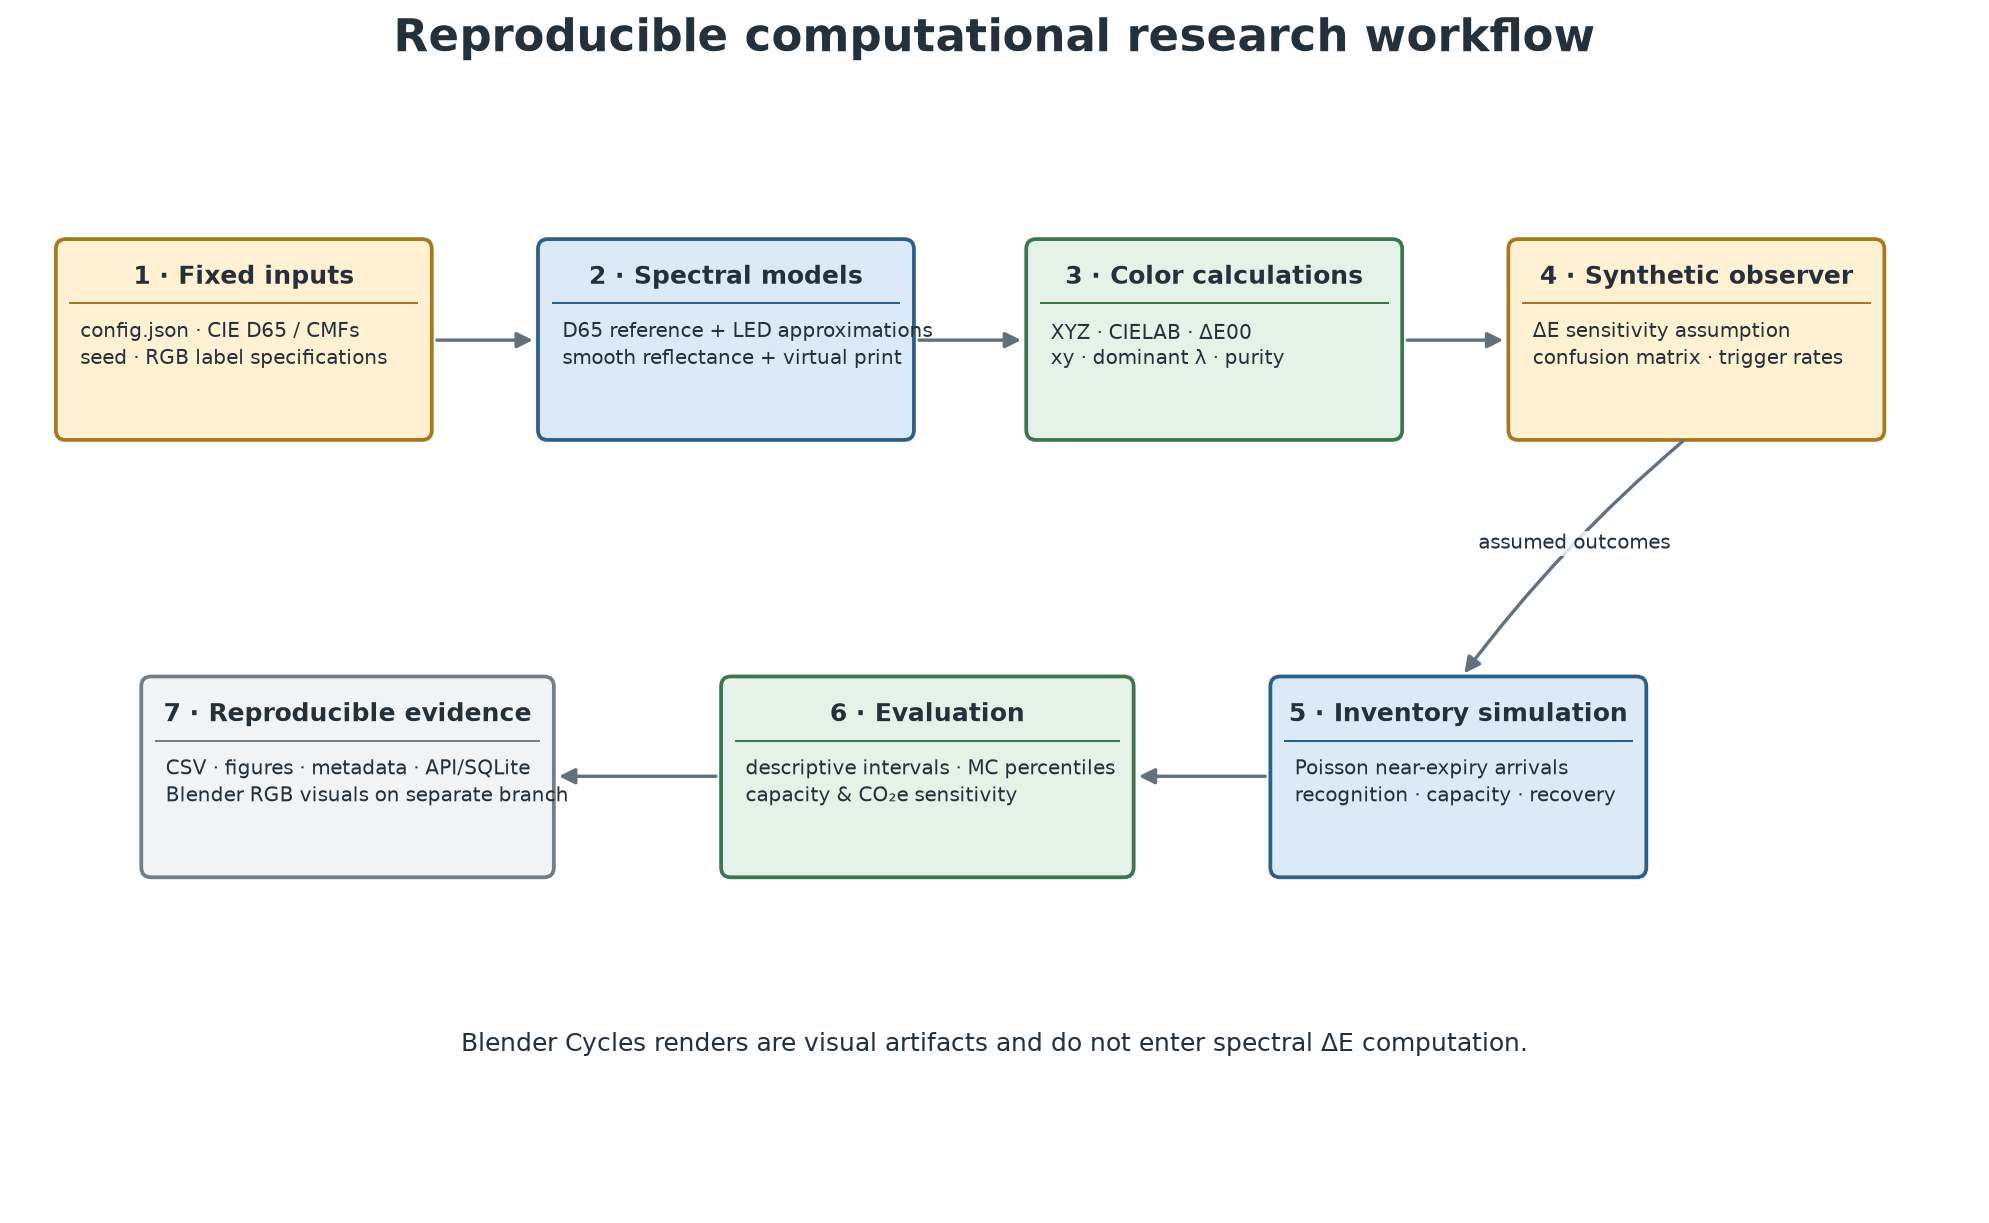
\includegraphics[width=\columnwidth]{research_methodology_flowchart.png}
\caption{Implemented sequence from configuration and CIE tables to calculations, simulated outcomes, and evidence.}
\label{fig:workflow}
\end{figure}
\begin{figure}[!t]\centering
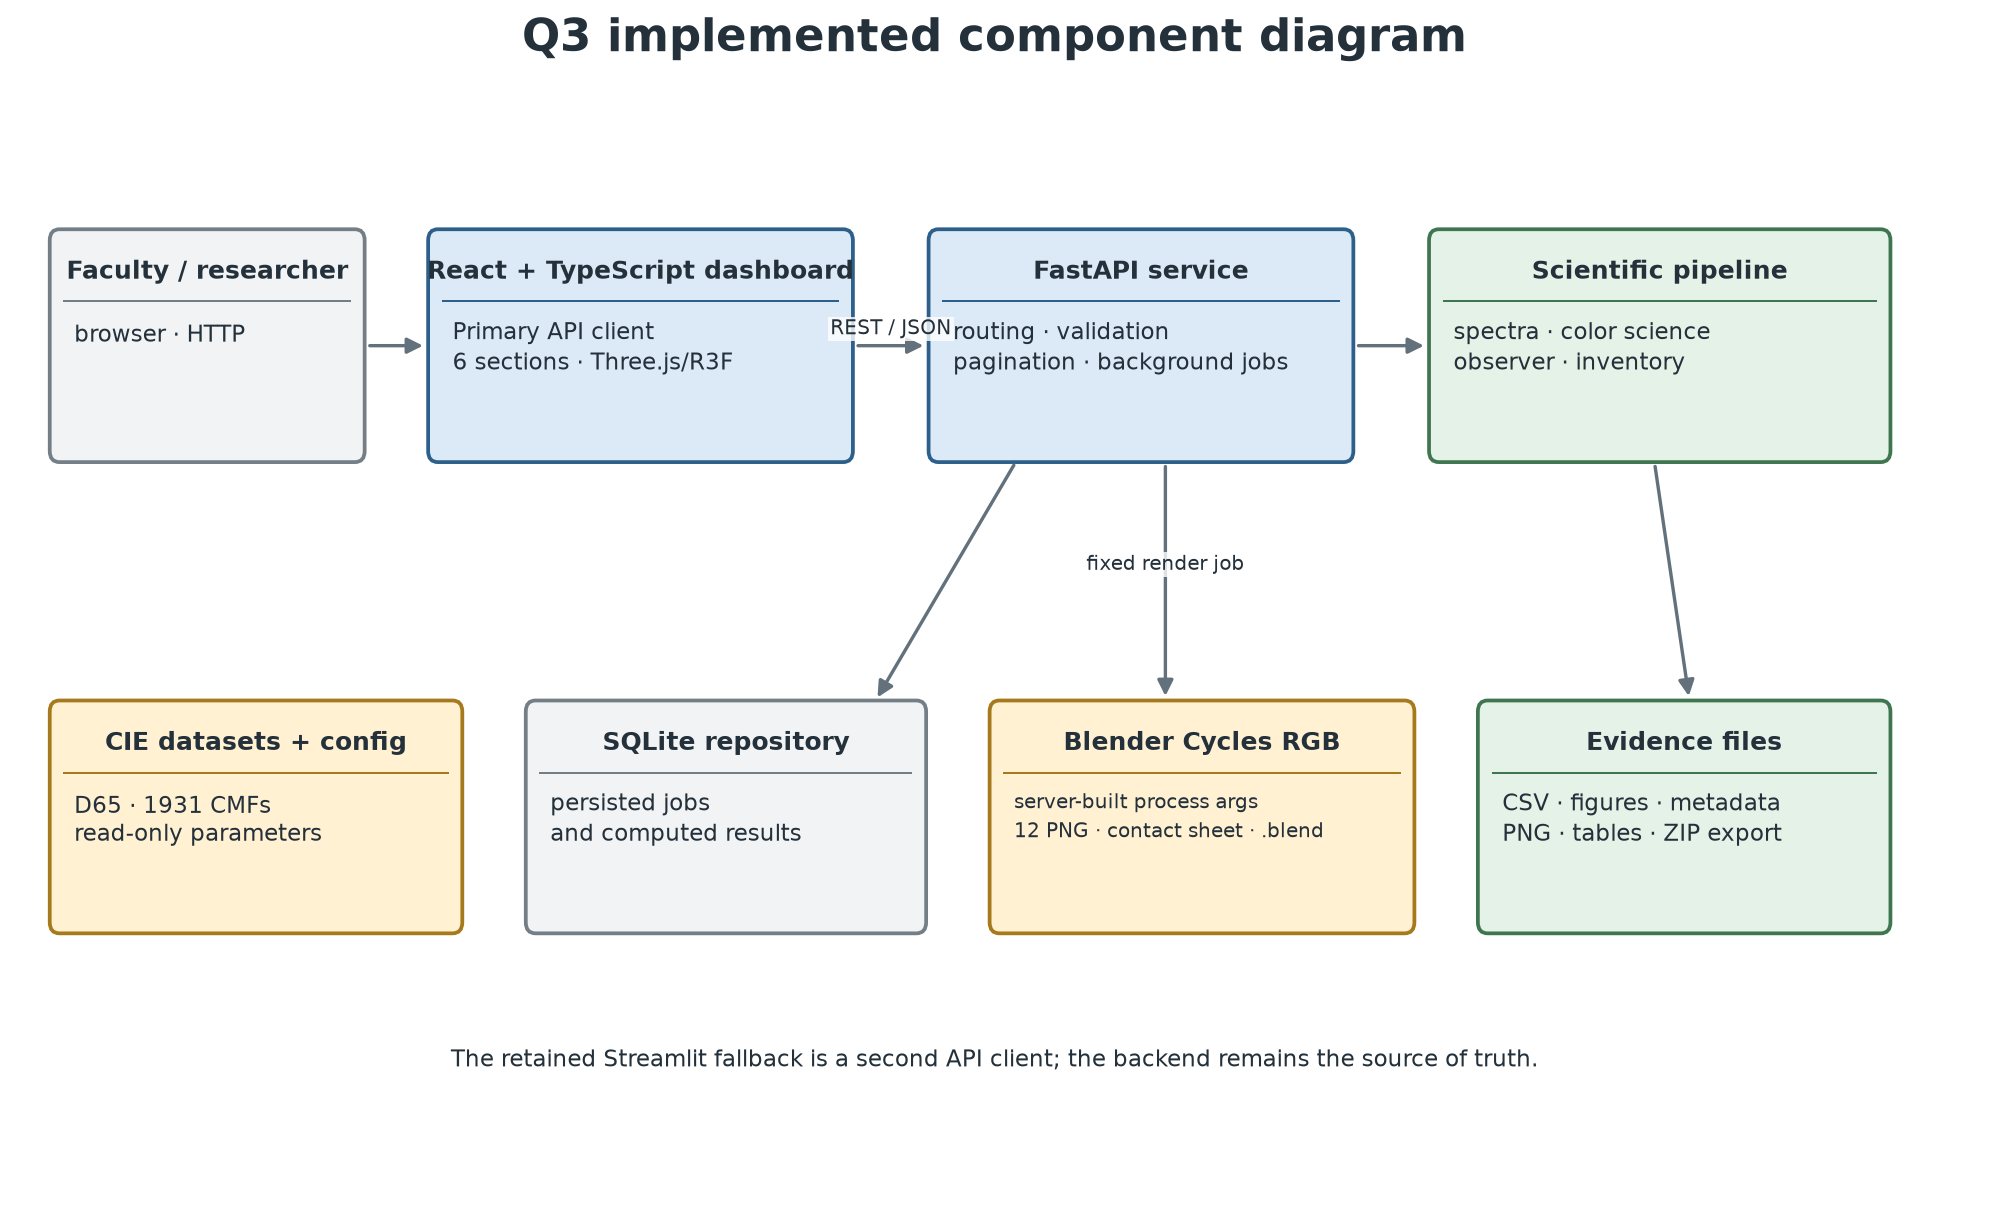
\includegraphics[width=\columnwidth]{component_diagram.png}
\caption{Implemented components. Blender provides RGB assets; Python provides numerical colour results.}
\label{fig:components}
\end{figure}

\subsection{Object design and operating-system modes}
Pydantic boundary models include \texttt{RenderJobRequest}, \texttt{ColourComparisonRequest}, \texttt{DonationSimulationRequest}, and \texttt{ObserverParameters}. Numerical methods remain focused functions in \texttt{colour\_engine} and \texttt{simulation}; SQLite persistence isolates parameterized queries and transactions. UML class and object diagrams are included; the object diagram depicts a runtime comparison, not a second class diagram.

Blender, Python, FastAPI, the browser, and SQLite run in user space. They request CPU, memory, files, and network through operating-system interfaces; the kernel performs privileged operations. No custom kernel module is needed because the project uses standard services and no bespoke device. Container controls can constrain a user-space process but do not move research logic into kernel mode.

SQLite stores render/analysis jobs, comparisons, and donation runs with IDs, status, request/results, errors, and timestamps. Connections commit successful operations and roll back on exceptions. The browser displays backend values and does not duplicate scientific calculations.

\section{Computational Methodology}
\subsection{Configuration and Blender scenes}
The configuration fixes Green/Fresh \texttt{\#2E9E4F}, Yellow/Watch \texttt{\#F5B700}, Orange/Discount \texttt{\#F07C1E}, and Red/Donate \texttt{\#D62828}. L1 is tabulated CIE D65 at nominal 6504 K. L2 and L3 are LED approximations targeting 4000 K and 3000 K. Calculations use 380--780 nm at 1-nm steps and the CIE 1931 2-degree observer.

The scenes were generated with Blender 5.2.3 LTS \cite{blender}. The controlled scene \texttt{q3\_project.blend} includes label, shelf/holder, grey reference card, camera, and scenario illumination panel. The label uses a controlled Diffuse BSDF connected to Material Output. Cycles renders use 8 samples, denoising, 960 by 640 pixels, and Standard view transform. Blender output is RGB visualization; Python evaluates the spectra.

The separate presentation scene \texttt{q3\_supermarket.blend} contains four stocked aisles, fixtures, produce and chilled displays, checkout and architectural details, and 608 linked product assemblies across 12 generated package families. Six camera views cover the store, shelf, red warning macro, four-colour rail, illuminant appearance, and isometric view. Final images are 2560 by 1440 Cycles CPU renders with OpenImageDenoise and AgX Medium High Contrast. Blackbody/emission nodes and area-light proxies are for presentation, not authoritative SPDs. The exported featured-shelf GLB supports browser viewing only. The six presentation views and twelve controlled RGB renders appear in Figs.~\ref{fig:supermarket} and~\ref{fig:conditions}.

\begin{figure*}[!t]\centering
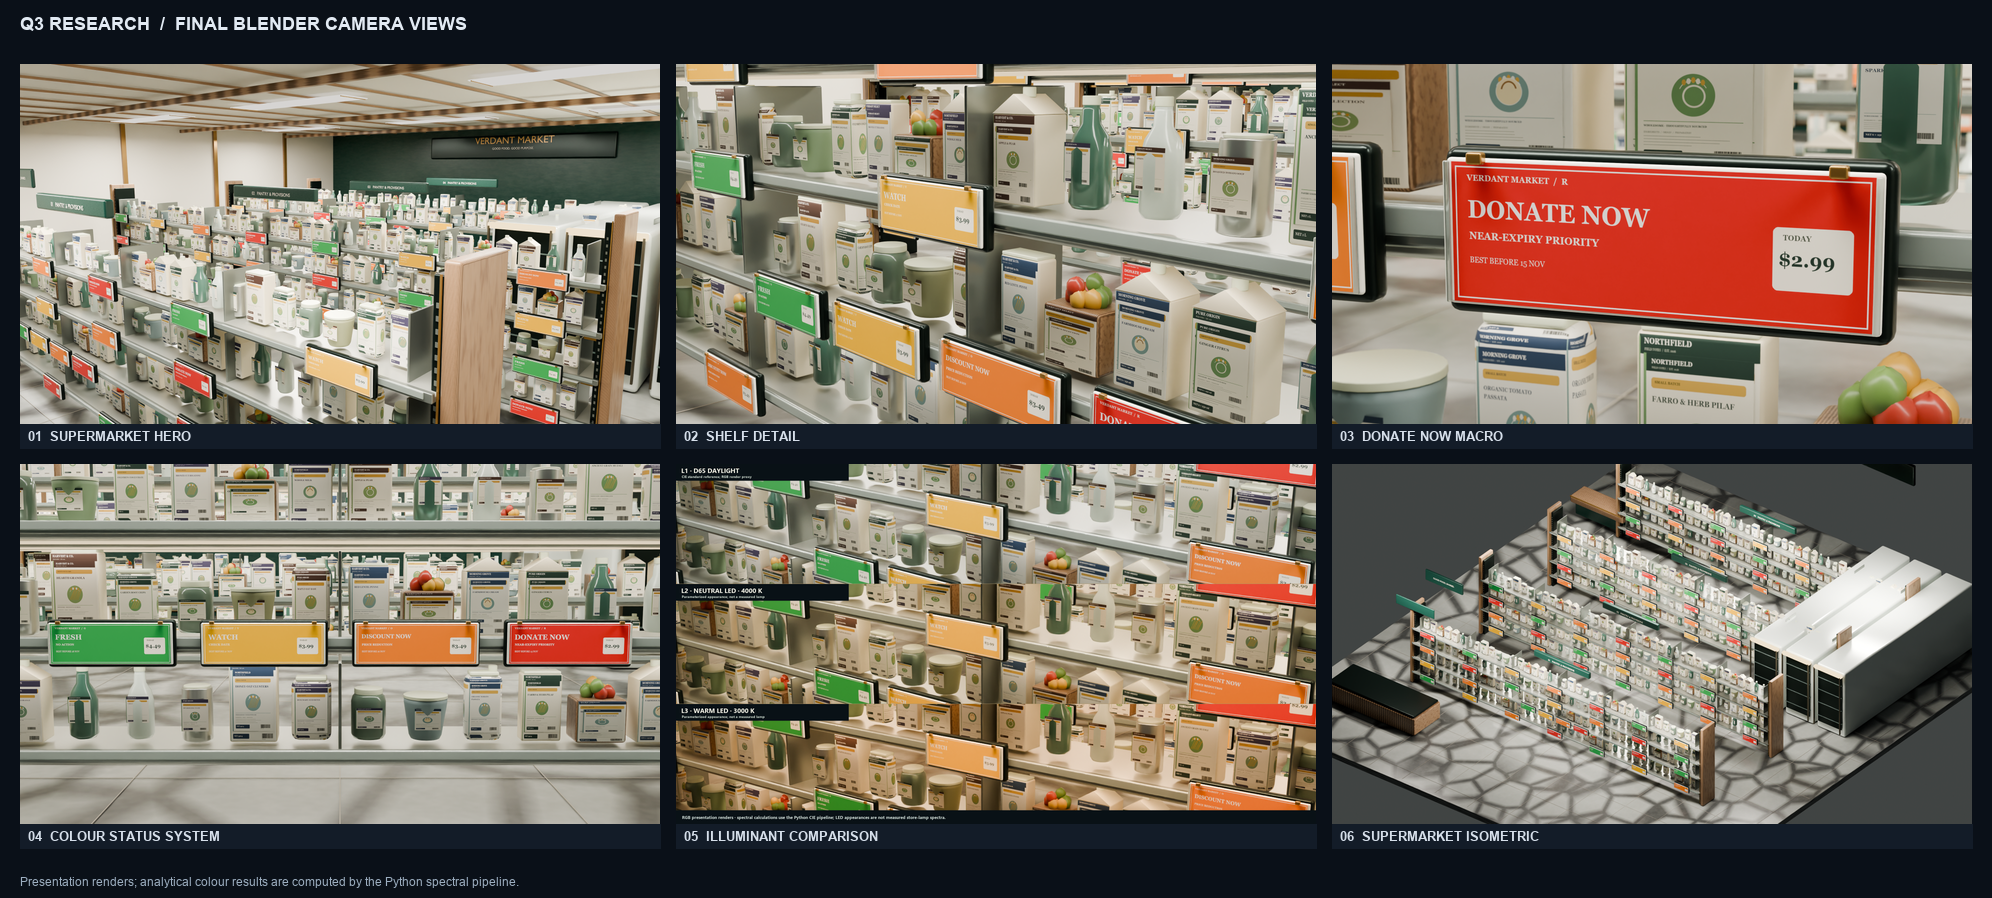
\includegraphics[width=0.96\textwidth]{supermarket_six_views_plate.png}
\caption{Six production camera views composed from saved Blender renders. They show retail context and are not measurement images.}
\label{fig:supermarket}
\end{figure*}
\begin{figure}[!t]\centering
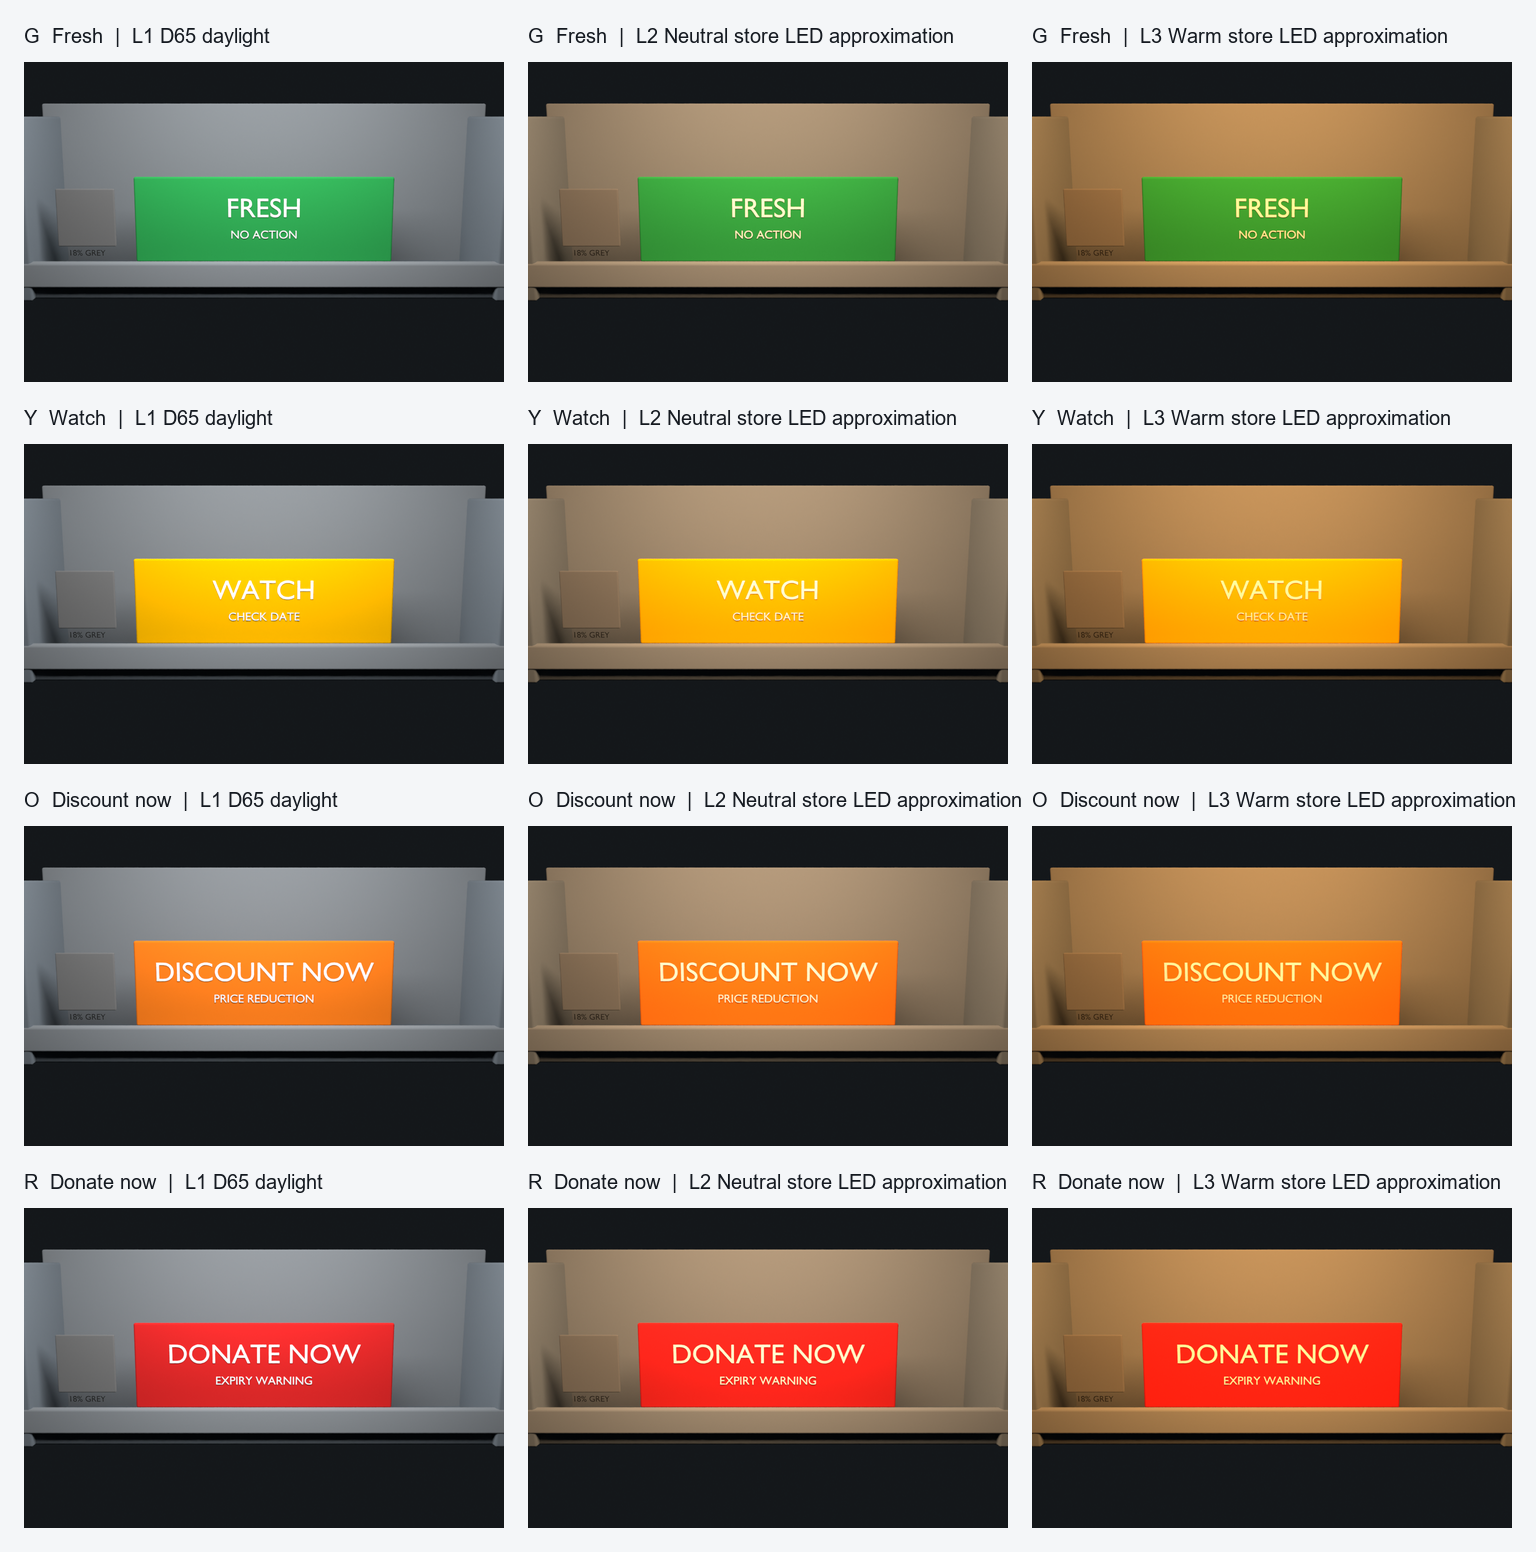
\includegraphics[width=\columnwidth]{12_condition_contact_sheet.png}
\caption{Twelve controlled RGB Cycles renders: four label colours under three visual lighting conditions. Analytical values come from Python, not render pixels.}
\label{fig:conditions}
\end{figure}

\subsection{Illumination and reflectance reconstruction}
For encoded sRGB component $c_s\in[0,1]$, IEC decoding is
\begin{equation}
c=\begin{cases}c_s/12.92,&c_s\leq0.04045,\\
((c_s+0.055)/1.055)^{2.4},&c_s>0.04045.\end{cases}
\end{equation}
Linear RGB is transformed to D65 XYZ using the IEC sRGB matrix:
\begin{equation}
\begin{bmatrix}X\\Y\\Z\end{bmatrix}=
\begin{bmatrix}
0.4124564&0.3575761&0.1804375\\
0.2126729&0.7151522&0.0721750\\
0.0193339&0.1191920&0.9503041
\end{bmatrix}
\begin{bmatrix}R\\G\\B\end{bmatrix}.
\end{equation}
Three tristimulus values do not determine a unique spectrum, so code selects a smooth bounded metamer:
\begin{align}
\mathbf r^*&=\arg\min_{\mathbf r\in[0.005,0.995]^{401}}J(\mathbf r),\\
J(\mathbf r)&=25^2\|M\mathbf r-\mathbf t\|_2^2
 +0.8^2\|D_2\mathbf r\|_2^2\nonumber\\
&\quad+0.015^2\|\mathbf r-0.72\mathbf 1\|_2^2.
\end{align}
where $\mathbf r$ has 401 wavelength samples, $\mathbf t$ is target linear-sRGB XYZ, $M$ is the D65/CIE-observer integration matrix, and $D_2$ is the second-difference operator. This regularization selects one solution; it does not infer physical ink or substrate spectra.


For illuminant $j$ and reflectance $R(\lambda)$,
\begin{align}
X&=K\sum_\lambda S_j(\lambda)R(\lambda)\bar x(\lambda)\Delta\lambda,\\
Y&=K\sum_\lambda S_j(\lambda)R(\lambda)\bar y(\lambda)\Delta\lambda,\\
Z&=K\sum_\lambda S_j(\lambda)R(\lambda)\bar z(\lambda)\Delta\lambda,
\end{align}
where $K=100/\sum_\lambda S_j(\lambda)\bar y(\lambda)\Delta\lambda$ sets a perfect diffuser to $Y=100$. CSV XYZ values are divided by 100, so a perfect diffuser has $Y=1$.

The LED engine combines three Gaussian bands centred at 450, 555, and 615 nm with standard deviations 17, 72, and 48 nm. Nonnegative weights are fitted to the chromaticity of a Planckian target at the configured CCT; the spectrum is normalized to 100 at 560 nm. CCT and chromaticity do not uniquely specify an SPD. Neither model represents a measured retail lamp.

\subsection{Virtual print-response model}
The synthetic response uses relative absorbance $A(\lambda)=-\ln(\max(R(\lambda),0.005))$. Define the blue-bias term
\begin{equation}
G(\lambda)=\exp\!\left[-\frac{(\lambda-455\,\mathrm{nm})^2}{2(45\,\mathrm{nm})^2}\right].
\end{equation}
Then, with $H(\lambda)=-1.06A(\lambda)-0.018G(\lambda)$,
\begin{equation}
R^p(\lambda)=\operatorname{clip}\!\left(0.96e^{H(\lambda)},\,0.005,\,0.995\right).
\end{equation}
\Needspace{4\baselineskip}
Configured virtual-print values are substrate multiplier 0.96, density gain 1.06, and blue absorbance bias 0.018 (Gaussian $\mu=455$ nm, $\sigma=45$ nm). This is not an ICC profile or printer measurement; the selected metamer and parameters affect the result.

\subsection{CIELAB, CIEDE2000, and chromaticity}
CIELAB uses the perfect-diffuser white under the relevant illuminant; no chromatic adaptation is applied between illuminants. For $t\geq0$, define $f(t)=t^{1/3}$ when $t>(6/29)^3$, and $f(t)=t/[3(6/29)^2]+4/29$ otherwise. Then
\begin{align}
L^*&=116f(Y/Y_n)-16,\nonumber\\
a^*&=500[f(X/X_n)-f(Y/Y_n)],\nonumber\\
b^*&=200[f(Y/Y_n)-f(Z/Z_n)].
\end{align}
Here $(X_n,Y_n,Z_n)$ is the perfect-diffuser white for that illuminant. CIEDE2000 uses $k_L=k_C=k_H=1$. Let $u_L=\Delta L'/S_L$, $u_C=\Delta C'/S_C$, and $u_H=\Delta H'/S_H$; then
\begin{equation}
\dE=\sqrt{u_L^2+u_C^2+u_H^2+R_Tu_Cu_H}.
\end{equation}
The primed terms include chroma correction and hue wrapping; $S_L,S_C,S_H$ are weighting functions and $R_T$ is the blue-region rotation term. The implementation retains signed $\Delta L^*$ and raw $\Delta C^*_{ab}$ separately from adjusted $\Delta C'$ and $\Delta H'$. It is verified against bundled Sharma reference cases.

Chromaticity is $x=X/(X+Y+Z)$ and $y=Y/(X+Y+Z)$. Dominant wavelength is the intersection of a ray from the illuminant white through the sample with the CIE 1931 spectral locus. Excitation purity is sample-to-white distance divided by white-to-locus-intersection distance. Purple-line cases use complementary wavelength. These are geometric descriptors from computed tristimulus data, not independent observations.

\subsection{Reproducibility}
Configuration fixes seed 20261115, source tables, wavelengths, colours, assumptions, and simulation counts. Metadata records software versions and data checksums. CIE tables are sourced; LED spectra, reconstructed reflectances, print responses, and downstream outputs are calculated or simulated. No render pixel was used as a spectral measurement.

\section{Donation-Trigger and Near-Expiry Simulation}
\subsection{Synthetic observer}
For colour difference $\dE$, the assumed error probability is
\begin{equation}
z=\frac{\dE-m}{s},\qquad p_e(\dE)=p_0+p_{\max}\sigma(z),
\end{equation}
where $\sigma(z)=(1+\exp(-z))^{-1}$, $p_0=0.01$, $p_{\max}=0.39$, $m=8$, and $s=3$ in the recorded configuration.
Action order is Fresh, Watch, Discount, Donate. Conditional on error, alternatives receive relative weights 0.70 if adjacent and 0.15 if non-adjacent, then are normalized. The model generates 10,000 classifications per colour--illuminant condition using recorded pseudorandom seeds. A missed trigger is a true red label classified as a non-donation action; a false trigger is a non-red item classified as Donate. This probability curve and confusion pattern are assumptions, not participant-calibrated values.

\subsection{Inventory and capacity model}
Daily arrivals are $N_t\sim\operatorname{Poisson}(80)$. A multinomial allocation assigns half to red candidates and distributes the remainder evenly across the other labels. Under simulated errors, each true class is mapped through its \dE-dependent confusion row. Given predicted donation count $\widehat N_{D,t}$ and capacity $C$,
\begin{align}
D_t&=\min(\widehat N_{D,t},C),\\
B_t&=\max(0,\widehat N_{D,t}-D_t),\\
A_t&=\widehat N_{Discount,t}+B_t,\qquad
Q_t\mid A_t\sim\operatorname{Binomial}(A_t,0.55).
\end{align}
where $Q_t$ represents discount recovery, including overflow offered at discount. Residual expired stock is $E_t=\max(0,N_t-D_t-Q_t)$. The horizon is 30 days, $C\in\{10,25,50\}$ units/day, and there are 500 replicates per scenario. Perfect recognition is a model counterfactual; seed derivation is deterministic.

The reported units-saved metric is true-red donations plus discount-recovered units. False donations are recorded separately and consume capacity but are not credited as saved in this metric, although all donated units are excluded from the residual expired count. This accounting convention limits direct comparison of the two totals. Product age, food-safety eligibility, shelf-life distributions, prices, routing, cold-chain, and actual store processes are outside the model. It is an alternative scenario, not a reproduction of Nigam.

\subsection{Statistics and sensitivity}
Mean and sample standard deviation of \dE{} are calculated across the four fixed colours. Their 95\% $t$ intervals and paired illumination differences are descriptive for this finite design, not population inference. Wilson intervals summarize binomial Monte Carlo trigger proportions. Inventory intervals are 2.5th and 97.5th percentiles across 500 replicate outputs. A statsmodels logistic fit is retained as a diagnostic on assumption-generated trials; it is not an empirical behavioral effect, and no inferential $p$-value supports a human claim.


\section{Implementation and Software Testing}
\subsection{Application and API}
The recorded stack is Python 3.11.9, NumPy 2.4.6, Pandas 3.1.1, SciPy 1.15.3, statsmodels 0.15.0, Matplotlib 3.11.2, colour-science 0.4.7, FastAPI 0.163.1, and SQLite. The primary client is React/TypeScript built with Vite; Three.js/React Three Fiber and the Blender-exported GLB support interaction. Streamlit remains a fallback. Analytical values and actions are API-backed.

Versioned REST resources expose health/configuration, job submission/status/history, comparison create/retrieve/history, donation create/retrieve/history, dashboard summaries, allow-listed artifacts, and CSV/evidence exports. Collections use \texttt{limit} (default 50, range 1--200) and nonnegative \texttt{offset}. Job histories accept \texttt{status}; comparison history accepts \texttt{illumination\_id}; donation history accepts \texttt{illumination\_id} and \texttt{recognition}. Responses include total, limit, offset, and items. FastAPI generates OpenAPI and Swagger documentation.

Pydantic validates request shapes and bounds render samples, observer probabilities, simulation horizon, arrivals, capacity, replicate count, and request budget; unknown fields are rejected. Jobs persist queued/running/completed/failed states. SQLite uses parameterized SQL and transaction rollback. Unexpected errors are logged and returned as generic 500 responses. Application-level containment uses server-generated output paths, artifact allow-lists, no arbitrary upload or shell fragment, subprocess argument arrays/timeouts, and bounded simulation work. This is not a formal security certification.

\subsection{Testing evidence}
The retained Phase 4 backend log records 28 pytest tests passed and one Starlette/httpx deprecation warning. Tests cover colour conversion and CIEDE2000 cases, spectral and print constraints, simulation repeatability, validation, persistence, pagination, artifact access, and errors. The frontend log records 3 Vitest tests passed, and the TypeScript/Vite production build completed. The Playwright log records 3 end-to-end tests passed: all six application sections and exports with the live API; Blender PNG fallback when WebGL is unavailable; and a real 12-condition Blender render job. These logs evidence software workflows, not human acceptance results.

Dockerfile and Compose describe an unprivileged, volume-backed deployment with health checks. Docker execution and cloud deployment are not verified. No cloud availability, backup recovery, or service performance is claimed.

\section{Results and Analysis}
\subsection{Colour differences}
Table~\ref{tab:deltae} reports all 12 calculated values. Fig.~\ref{fig:deltae} visualizes the configured colour-by-illuminant differences. Mean \dE{} across four fixed labels is 2.1207 (SD 0.2669) under D65, 2.1042 (SD 0.3241) for the 4000-K LED approximation, and 2.0436 (SD 0.3813) for the 3000-K approximation. Descriptive 95\% intervals across the four labels are [1.6960,2.5453], [1.5884,2.6200], and [1.4368,2.6504]. The intervals overlap and do not support inferential illumination claims.

\begin{table*}[!t]
\caption{Calculated CIEDE2000 differences for all 12 configured conditions.}
\label{tab:deltae}\centering\small
\begin{tabular}{llrrr}
\toprule
Label & sRGB & D65 & Neutral LED & Warm LED \\
\midrule
Green / Fresh & \#2E9E4F & 2.4090 & 2.5309 & 2.5573 \\
Yellow / Watch & \#F5B700 & 1.9116 & 1.7433 & 1.6416 \\
Orange / Discount & \#F07C1E & 2.2856 & 2.0905 & 1.9401 \\
Red / Donate now & \#D62828 & 1.8765 & 2.0521 & 2.0355 \\
\bottomrule
\end{tabular}
\par\vspace{3pt}\footnotesize Each cell is one deterministic digital-metamer versus virtual-print calculation; these are not physical label measurements.
\end{table*}


\begin{figure}[!t]\centering
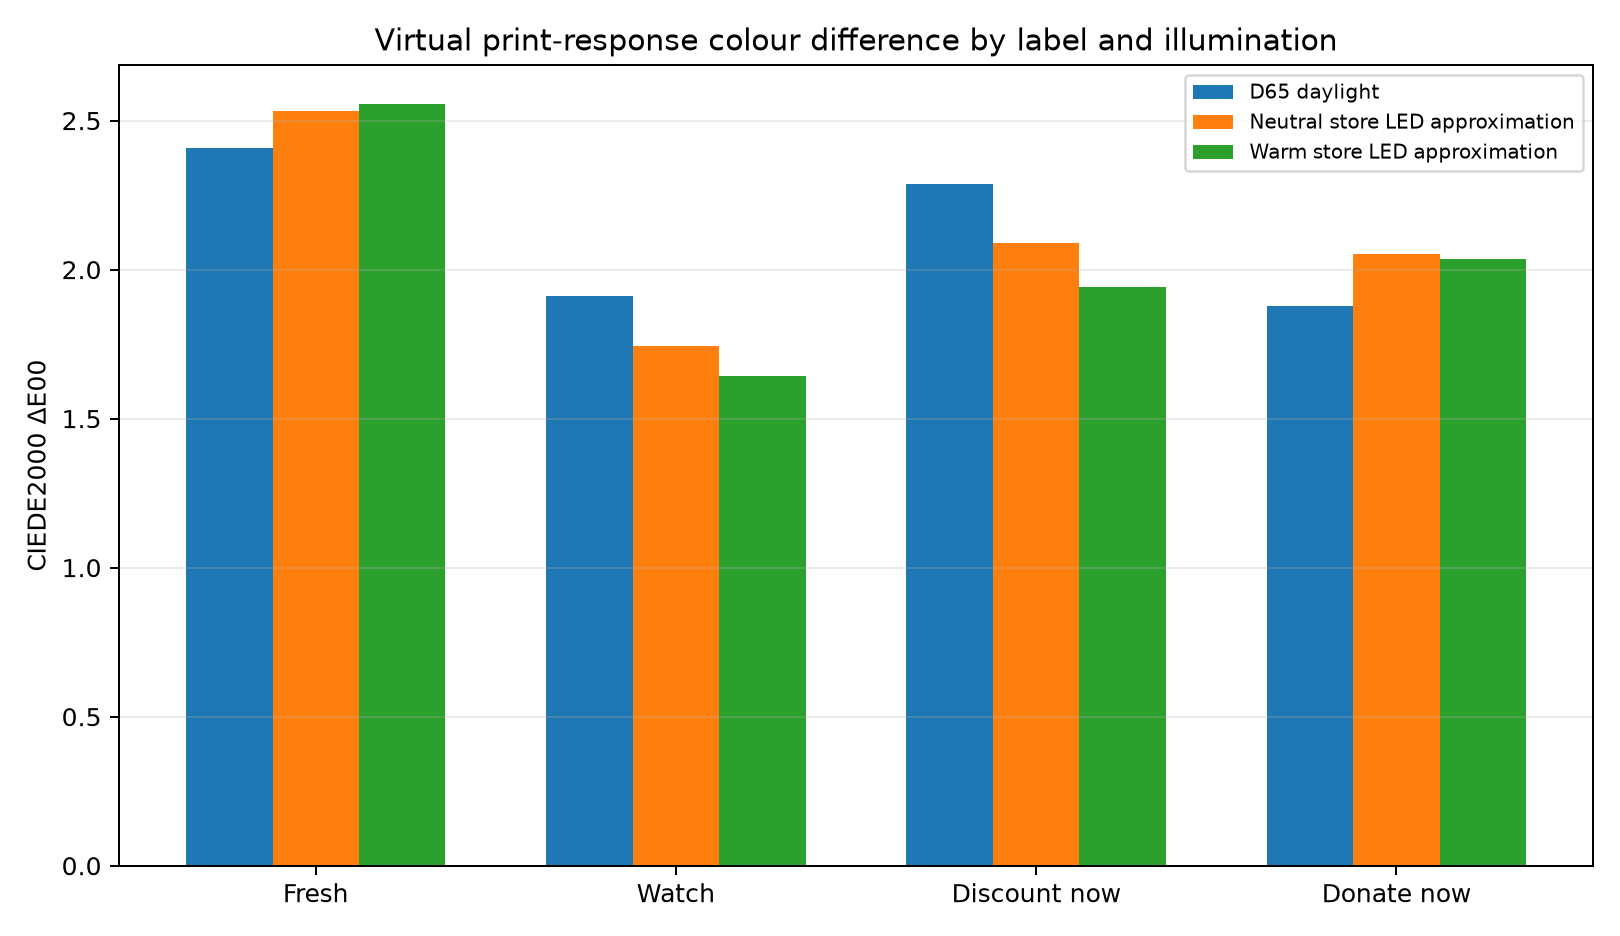
\includegraphics[width=\columnwidth]{delta_e_by_condition.png}
\caption{Calculated \dE{} by configured label and illuminant. One deterministic calculation per cell; no physical replicates.}
\label{fig:deltae}
\end{figure}

\subsection{Red DONATE NOW results}
For red \texttt{\#D62828}, \dE{} is 1.876517 under D65, 2.052059 under the neutral LED approximation, and 2.035453 under the warm LED approximation. Relative to D65, the computed differences increase by 0.175542 and 0.158936. These values compare the chosen digital metamer with a synthetic print response, not an actual printed label.

Table~\ref{tab:redcolour} gives the CIEDE2000 component terms, which are plotted in Fig.~\ref{fig:redcomponents}. Under D65, digital \Lab{} is $(46.942109,64.829019,44.486708)$ and virtual-print \Lab{} is $(45.004048,64.213273,43.809044)$. Digital red chromaticity is $(0.596311,0.329906)$; its dominant wavelength is 611.266607 nm and purity 0.794474 relative to D65 white. Fig.~\ref{fig:chromaticity} shows the computed chromaticity context. Under L2 and L3, digital wavelengths are 605.514329 nm and 606.572037 nm, and purities are 0.913689 and 0.928202 relative to each illuminant's white. Full XYZ, Lab, xy, and CIEDE2000 components for all cases remain in CSV files.

\begin{table*}[!t]
\caption{Primary red DONATE NOW colour result and CIEDE2000 component terms.}
\label{tab:redcolour}\centering\scriptsize
\begin{tabular}{lrrrrr}
\toprule
Illuminant & $\Delta E_{00}$ & $\Delta L^*$ & Raw $\Delta C^*_{ab}$ & Adjusted $\Delta C'$ & Adjusted $\Delta H'$ \\
\midrule
D65 & 1.8765 & -1.9381 & -0.8908 & -0.8909 & -0.2116 \\
4000-K LED model & 2.0521 & -2.0255 & -1.2923 & -1.2923 & -0.3696 \\
3000-K LED model & 2.0355 & -2.0748 & -1.2886 & -1.2886 & -0.2862 \\
\bottomrule
\end{tabular}
\par\vspace{3pt}\footnotesize Signed changes are virtual print minus digital. Raw $\Delta C^*_{ab}$ is distinct from the adjusted CIEDE2000 term.
\end{table*}


\begin{figure*}[!t]\centering
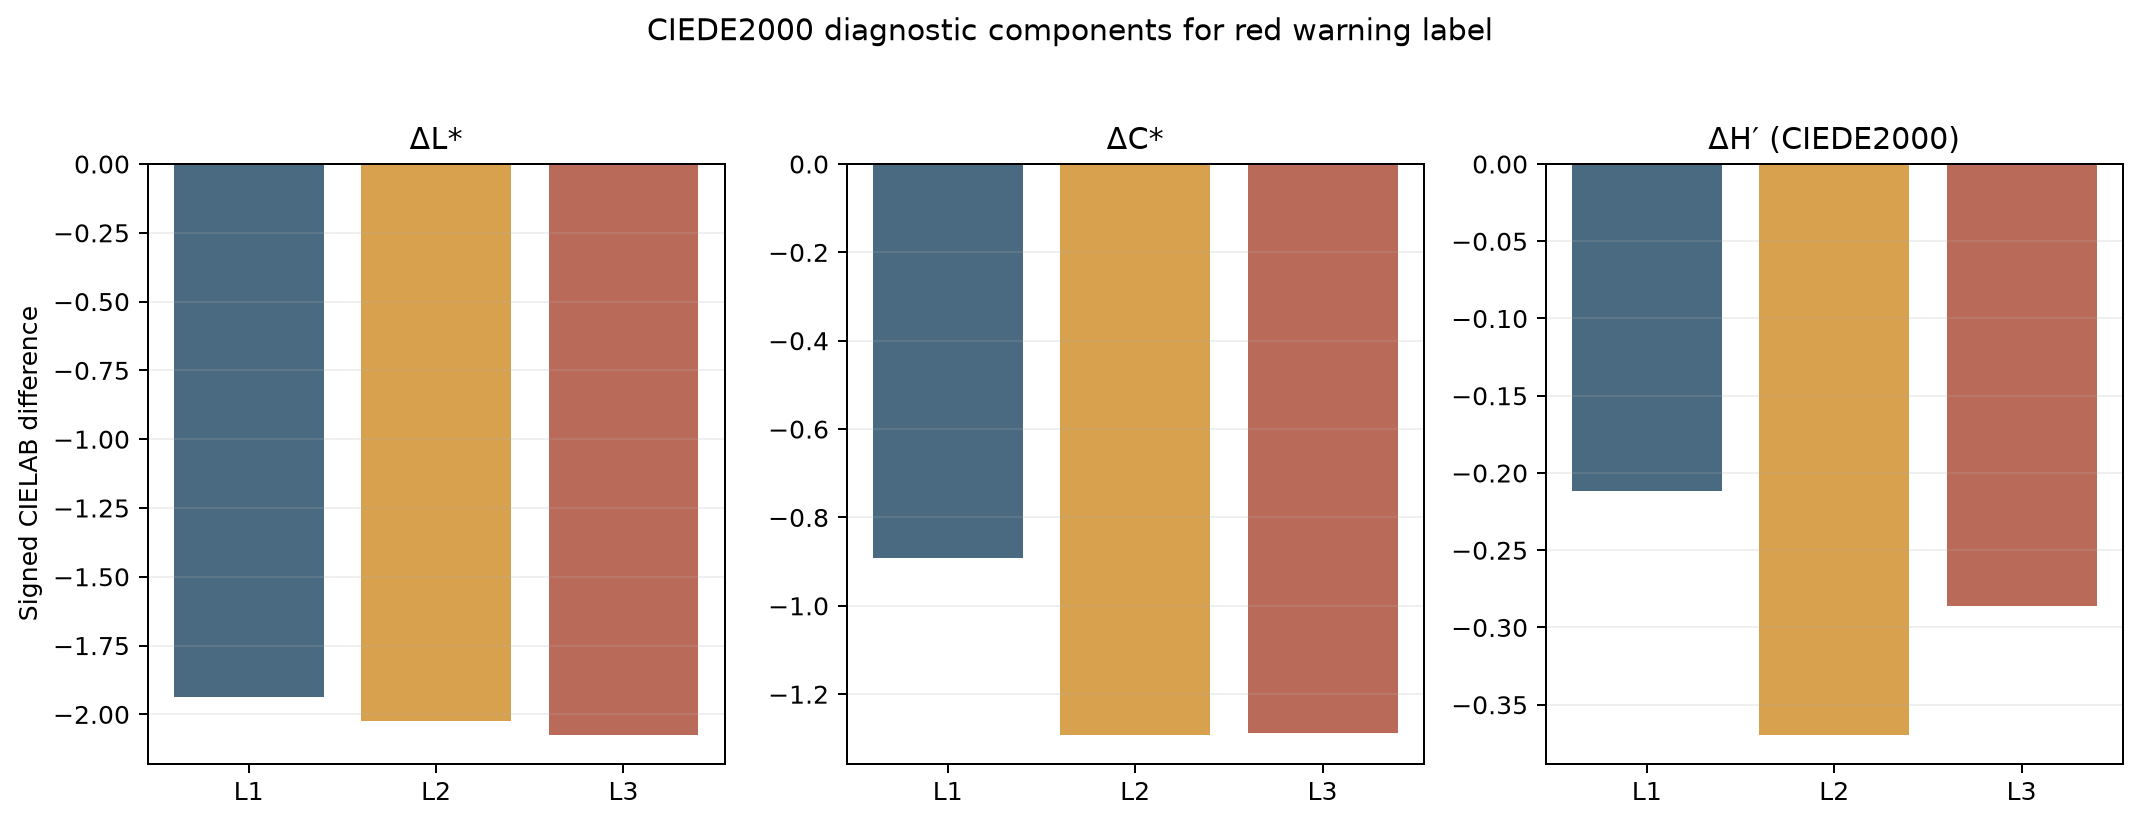
\includegraphics[width=0.96\textwidth]{red_delta_components.png}
\caption{Calculated red-label \dE{} components under the three modeled illuminants.}
\label{fig:redcomponents}
\end{figure*}
\begin{figure}[!t]\centering
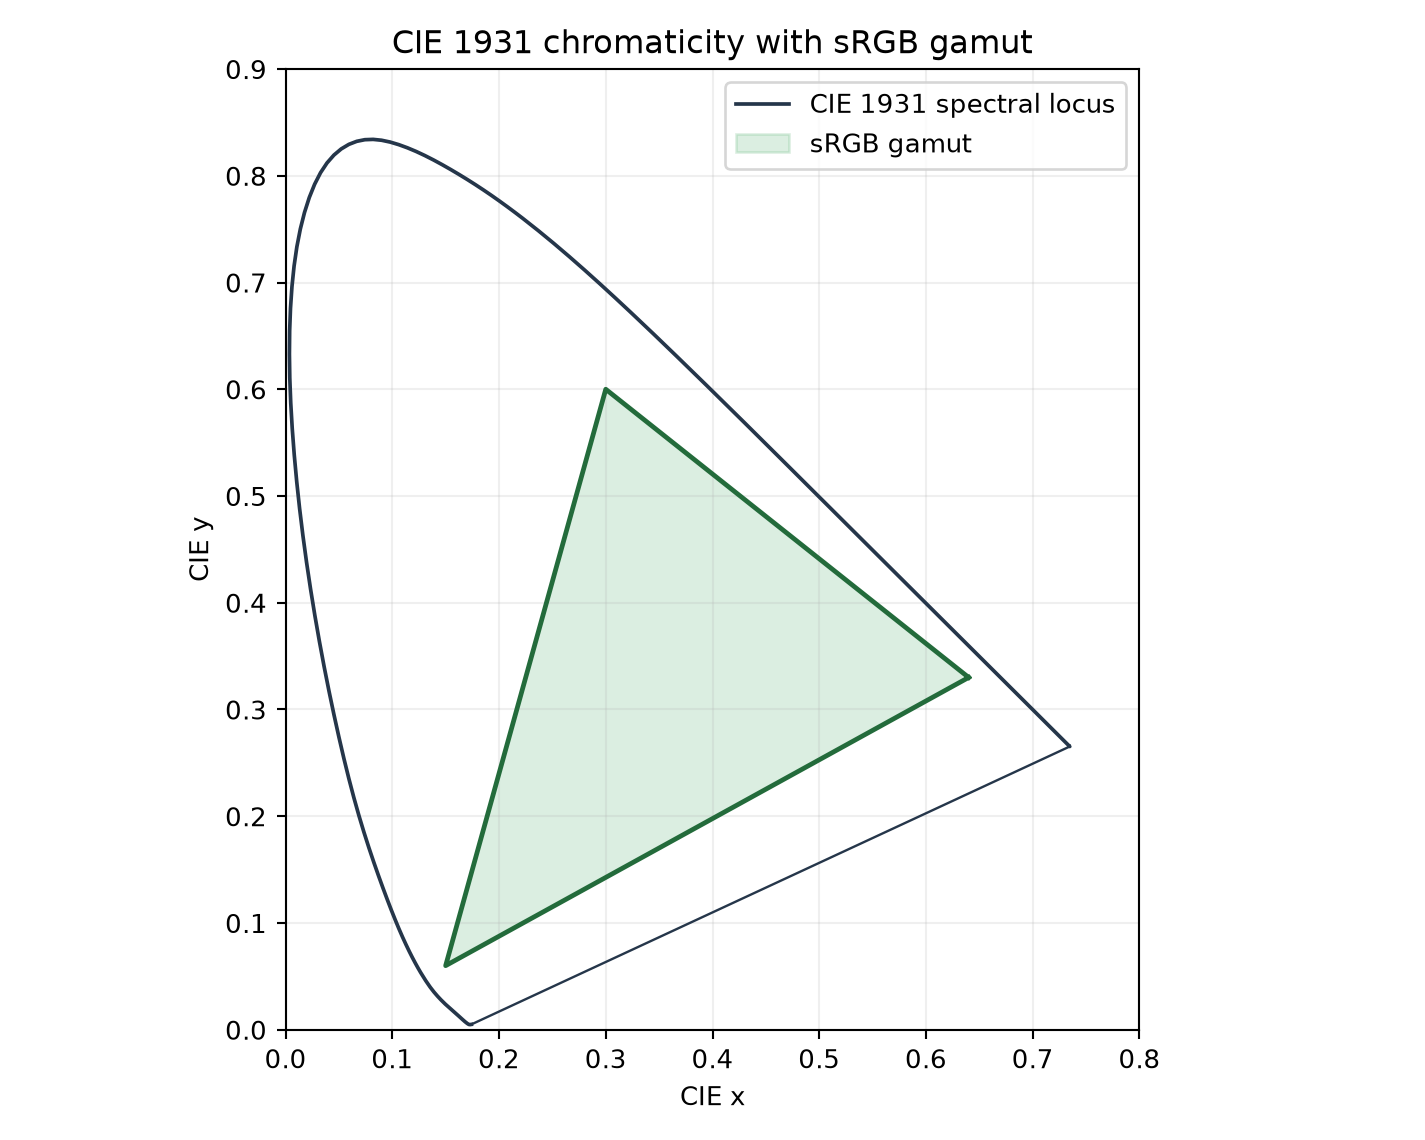
\includegraphics[width=\columnwidth]{cie1931_srgb_gamut.png}
\caption{CIE 1931 chromaticity diagram and sRGB gamut generated from project data. Configured points are calculated, not measured.}
\label{fig:chromaticity}
\end{figure}

\subsection{Simulated classifications}
Table~\ref{tab:triggers} reports the red-trigger counts and Wilson intervals. For true red labels, assumed error probabilities are 5.4830\%, 5.7204\%, and 5.6975\% under L1, L2, and L3. In 10,000 trials per condition, the model produces 546, 562, and 558 missed triggers. Wilson 95\% intervals are [5.0316,5.9226]\%, [5.1854,6.0887]\%, and [5.1469,6.0472]\%. These quantify finite random draws under the chosen model, not uncertainty about a human population. Fig.~\ref{fig:confusion} displays the generated action matrices; Fig.~\ref{fig:triggerdelta} shows the relationship imposed by the assumed sensitivity function. The descriptive logit coefficient is 0.279416 (SE 0.042976) on generated trials and is not evidence of behavioral prediction.

\begin{table*}[!t]
\caption{Simulated red-trigger misses under the configured observer model.}
\label{tab:triggers}\centering\small
\begin{tabular}{lrrrr}
\toprule
Illuminant & Assumed error probability & Misses / trials & Simulated miss rate & Wilson 95\% interval \\
\midrule
D65 & 5.4830\% & 546 / 10000 & 5.46\% & [5.032, 5.923]\% \\
4000-K LED model & 5.7204\% & 562 / 10000 & 5.62\% & [5.185, 6.089]\% \\
3000-K LED model & 5.6975\% & 558 / 10000 & 5.58\% & [5.147, 6.047]\% \\
\bottomrule
\end{tabular}
\par\vspace{3pt}\footnotesize Intervals quantify binomial Monte Carlo variation under the assumed synthetic observer, not human-population uncertainty.
\end{table*}


\begin{figure*}[!t]\centering
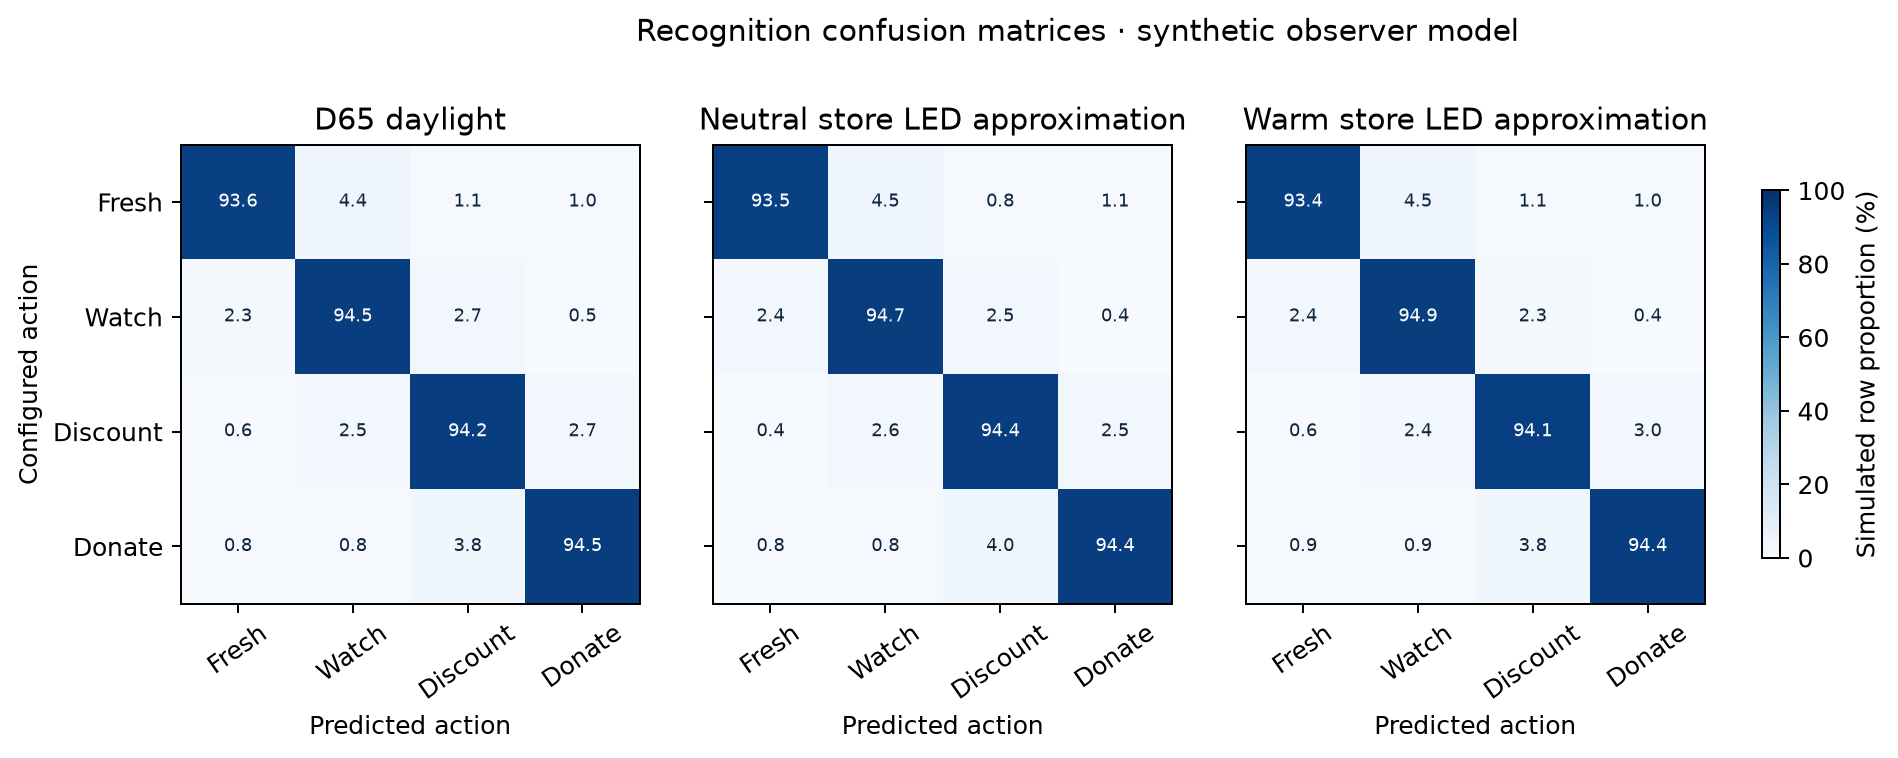
\includegraphics[width=0.96\textwidth]{recognition_confusion_matrices.png}
\caption{Confusion matrices from the assumed observer model, using its logistic error curve and action weights.}
\label{fig:confusion}
\end{figure*}
\begin{figure}[!t]\centering
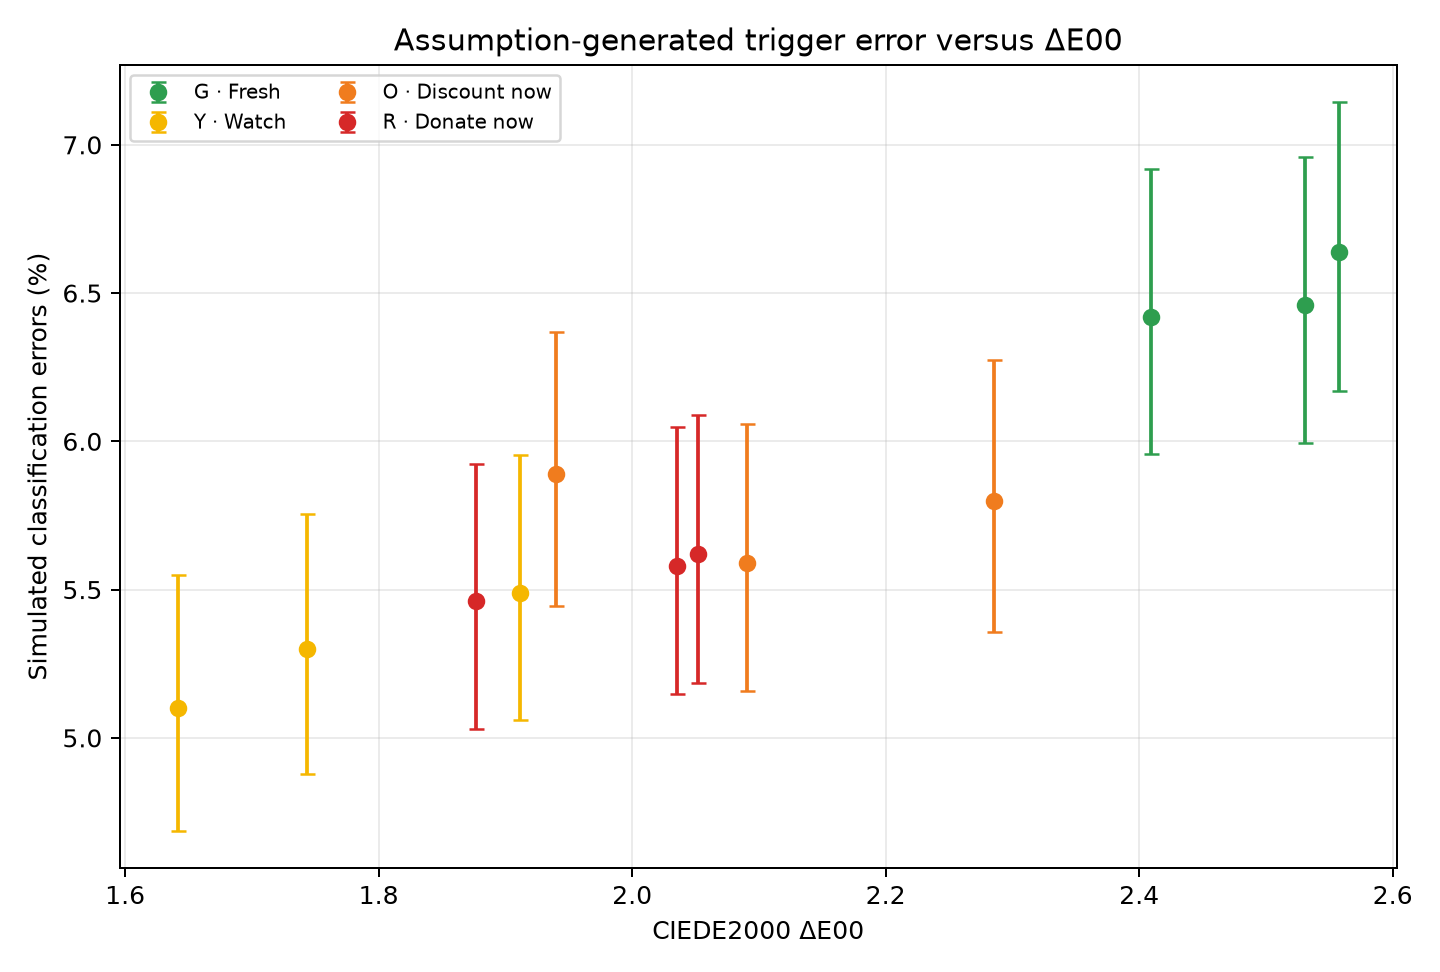
\includegraphics[width=\columnwidth]{trigger_error_vs_delta_e.png}
\caption{Generated classification error versus calculated \dE{}. The trend is imposed by the sensitivity function, not observed from people.}
\label{fig:triggerdelta}
\end{figure}


\subsection{Near-expiry outcomes and capacity}
Table~\ref{tab:donation} summarizes the D65 capacity scenarios. At L1 and capacity 25/day, perfect recognition saves a mean 1218.224 units (95\% replicate percentile interval 1169.950--1270.050) over 30 days. With simulated errors the mean is 1198.680 (1143.475--1251.000), a model difference of 19.544 units. Mean expired stock changes from 1181.628 to 1190.594; simulated errors produce means of 65.784 missed red triggers and 16.516 false donation triggers. Figs.~\ref{fig:donations} and~\ref{fig:capacity} compare inventory outcomes and capacity sensitivity. Mean units saved increase at larger capacities in both treatments under these assumptions.

\begin{table*}[!t]
\caption{Near-expiry Monte Carlo outcomes under D65 (500 replicates per scenario).}
\label{tab:donation}\centering\scriptsize
\begin{tabular}{llrrrrr}
\toprule
Recognition & Capacity/day & Saved units, mean [2.5th, 97.5th pct.] & Expired, mean & Missed triggers, mean & False triggers, mean & Waste rate \\
\midrule
Perfect & 10 & 1017.1 [967.0, 1073.0] & 1383.8 & 0.0 & 0.0 & 0.5764 \\
Perfect & 25 & 1218.2 [1170.0, 1270.0] & 1181.6 & 0.0 & 0.0 & 0.4923 \\
Perfect & 50 & 1417.6 [1345.5, 1485.5] & 982.1 & 0.0 & 0.0 & 0.4092 \\
Simulated errors & 10 & 1002.1 [947.5, 1053.5] & 1391.9 & 66.2 & 16.7 & 0.5803 \\
Simulated errors & 25 & 1198.7 [1143.5, 1251.0] & 1190.6 & 65.8 & 16.5 & 0.4960 \\
Simulated errors & 50 & 1370.7 [1299.0, 1437.5] & 1011.0 & 65.2 & 16.9 & 0.4215 \\
\bottomrule
\end{tabular}
\par\vspace{3pt}\footnotesize Saved-unit intervals are the 2.5th and 97.5th percentiles across 500 replicates; outcomes are modeled units, not observed stock.
\end{table*}

\begin{figure*}[!t]\centering
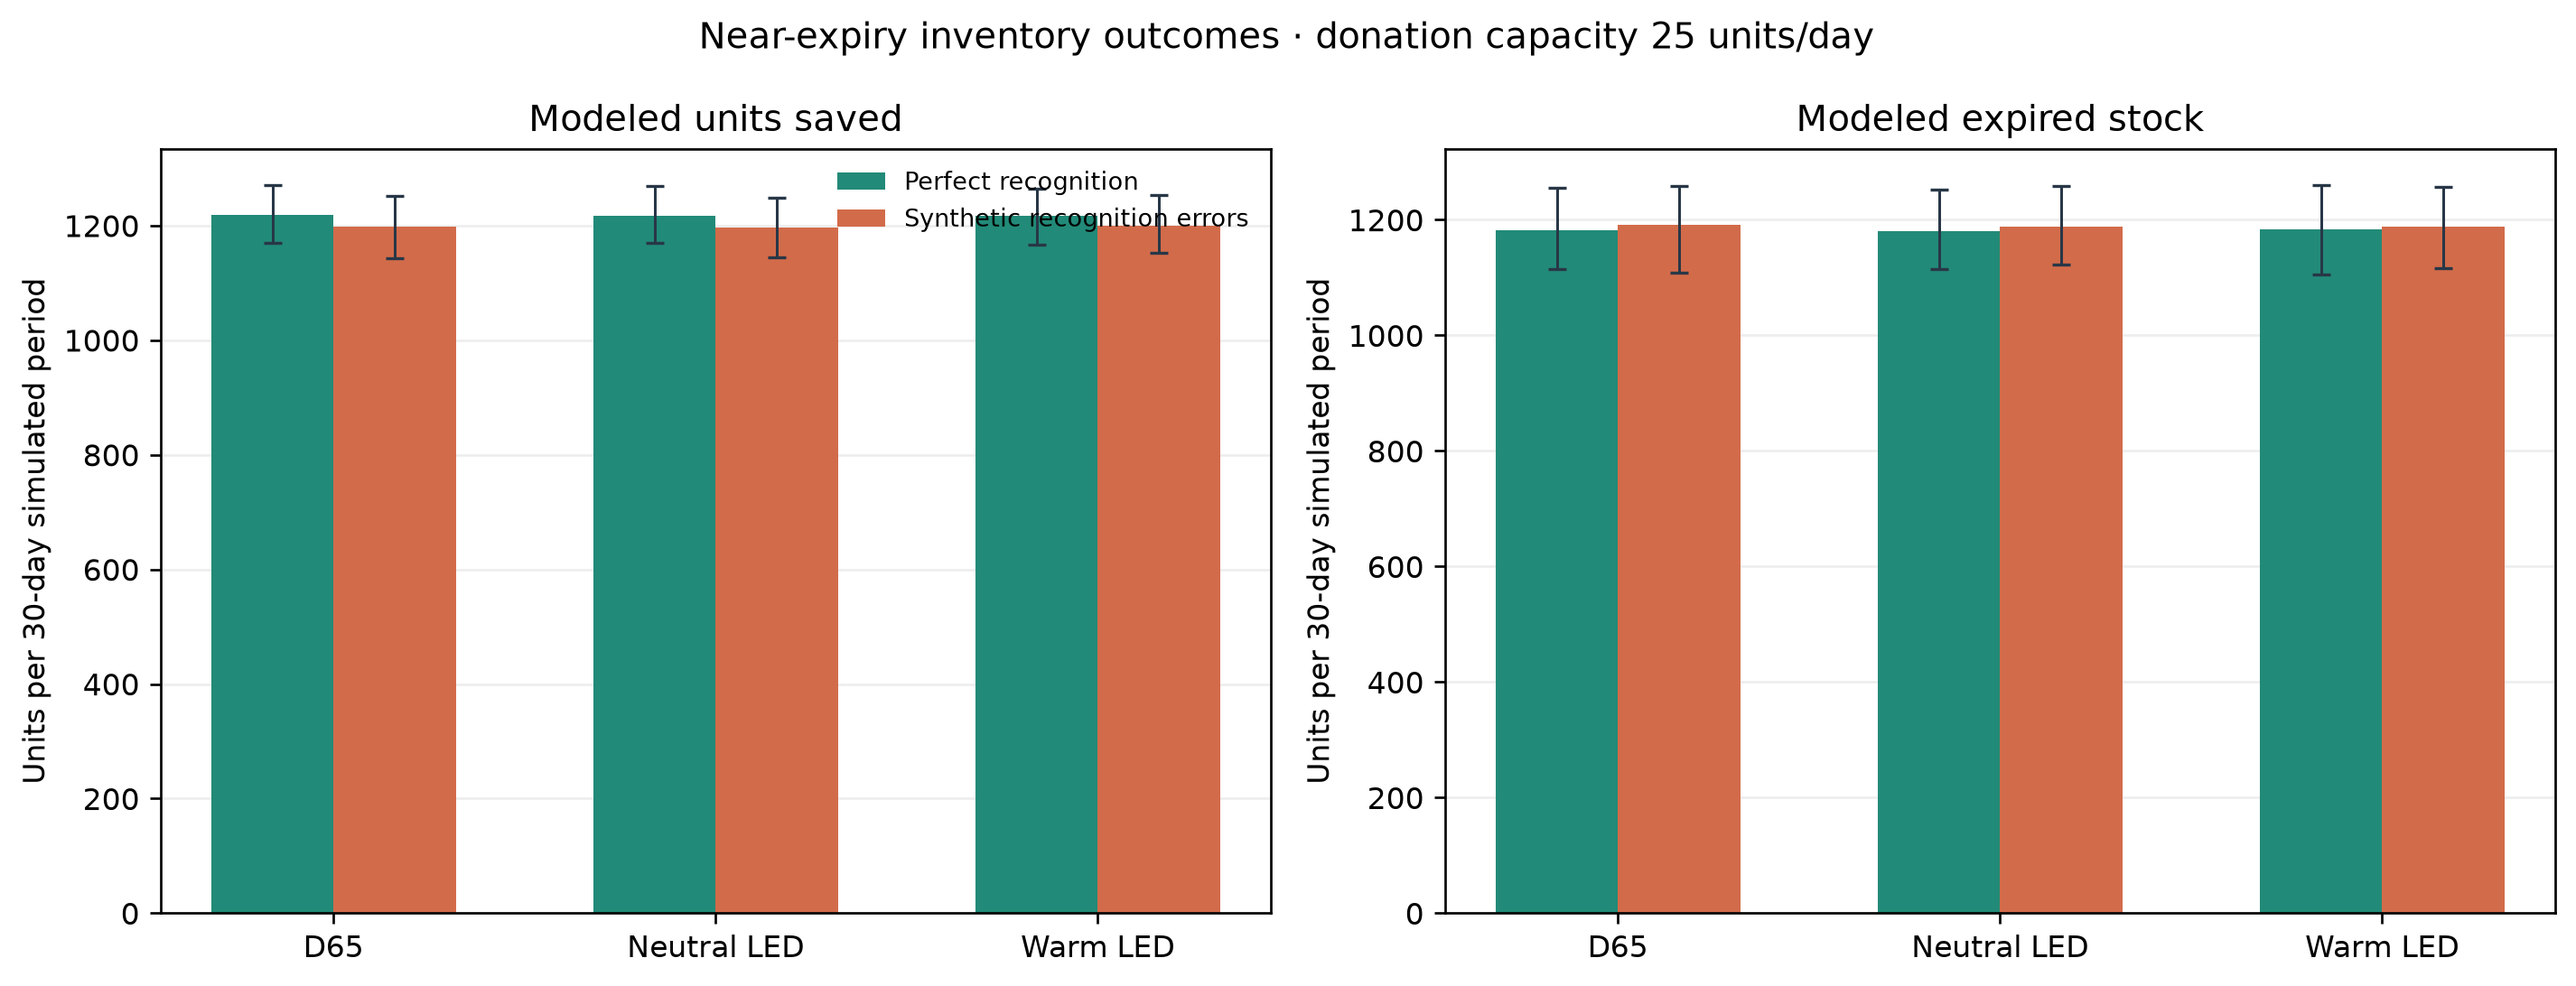
\includegraphics[width=0.96\textwidth]{near_expiry_simulation_comparison_paper.png}
\caption{Monte Carlo near-expiry outcomes under perfect recognition and simulated errors. Intervals summarize 500 model replicates per scenario.}
\label{fig:donations}
\end{figure*}
\begin{figure}[!t]\centering
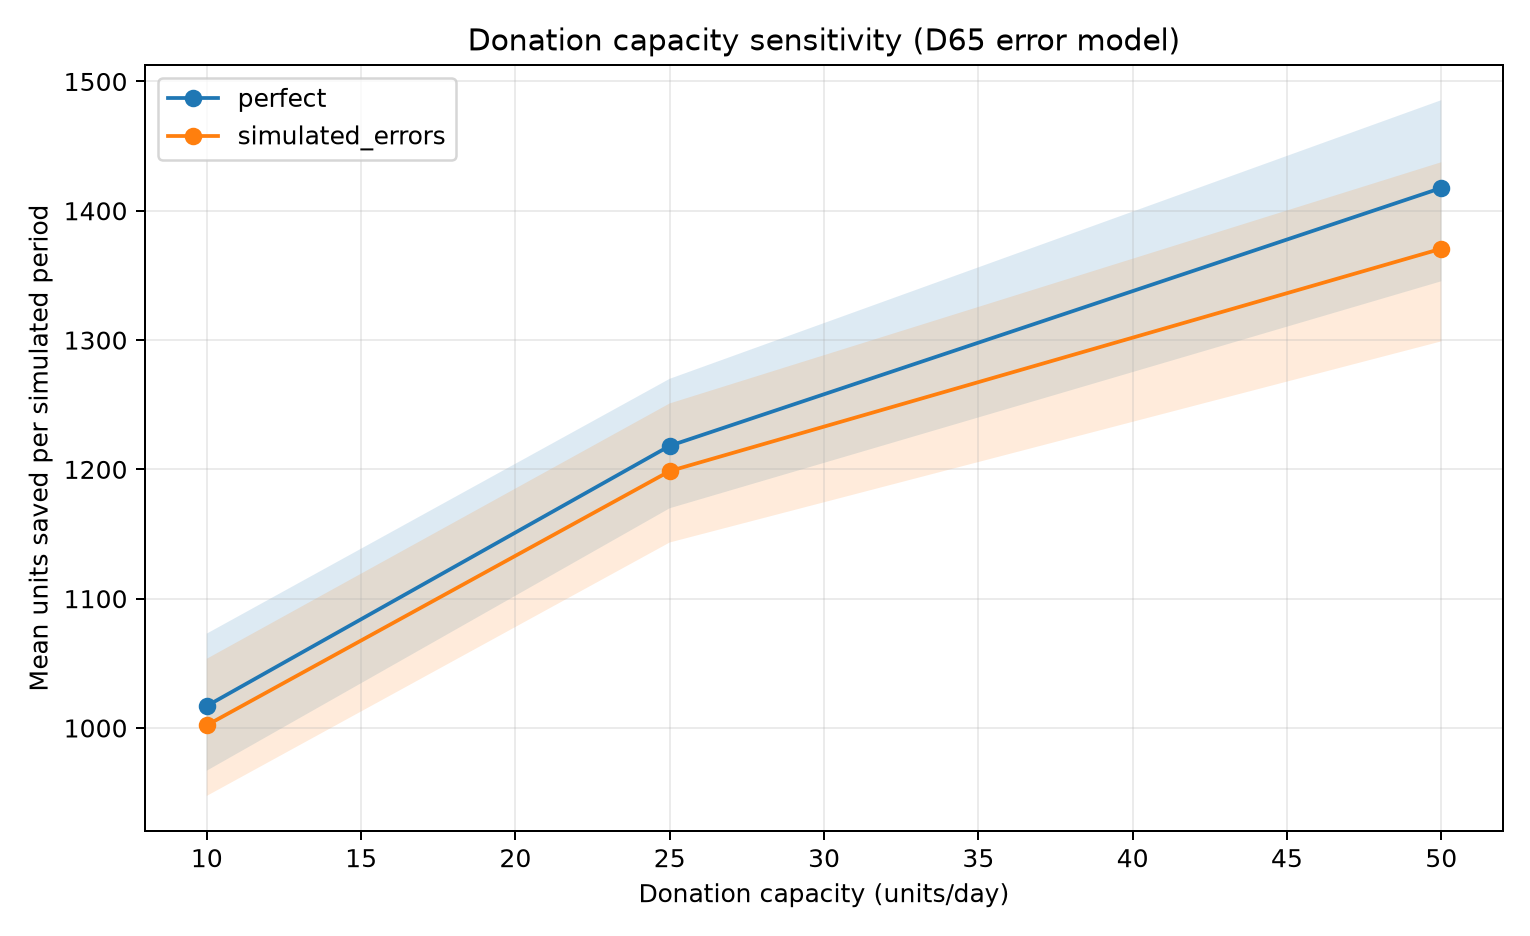
\includegraphics[width=\columnwidth]{donation_capacity_sensitivity.png}
\caption{Capacity sensitivity of the alternative inventory simulation; outcomes are modeled units, not observed retail stock.}
\label{fig:capacity}
\end{figure}

\subsection{Sustainability scenario}
For L1, simulated errors, and capacity 25/day, the 1198.680 mean saved units at an assumed 0.8 kg/unit correspond to 958.944 kg food mass. Table~\ref{tab:sustainability} and Fig.~\ref{fig:sustainability} show the low, central, and high scenarios: 1438.416, 2397.360, and 3356.304 kg CO$_2$e. The factors (1.5, 2.5, and 3.5 kg CO$_2$e/kg) are illustrative assumptions; no external emission factor was used. These are potential scenario estimates, not observed reductions, an LCA, or a Nigam score.

\begin{table}[!t]
\caption{Illustrative sustainability sensitivity for the L1, capacity-25 simulated-errors case.}
\label{tab:sustainability}\centering\footnotesize
\begin{tabular}{lrr}
\toprule
Factor scenario & kg CO$_2$e/kg & Modeled kg CO$_2$e \\
\midrule
Low & 1.5 & 1438.416 \\
Central & 2.5 & 2397.360 \\
High & 3.5 & 3356.304 \\
\bottomrule
\end{tabular}
\par\vspace{3pt}\footnotesize Factors are illustrative assumptions, not sourced product emission factors.
\end{table}

\begin{figure*}[!t]\centering
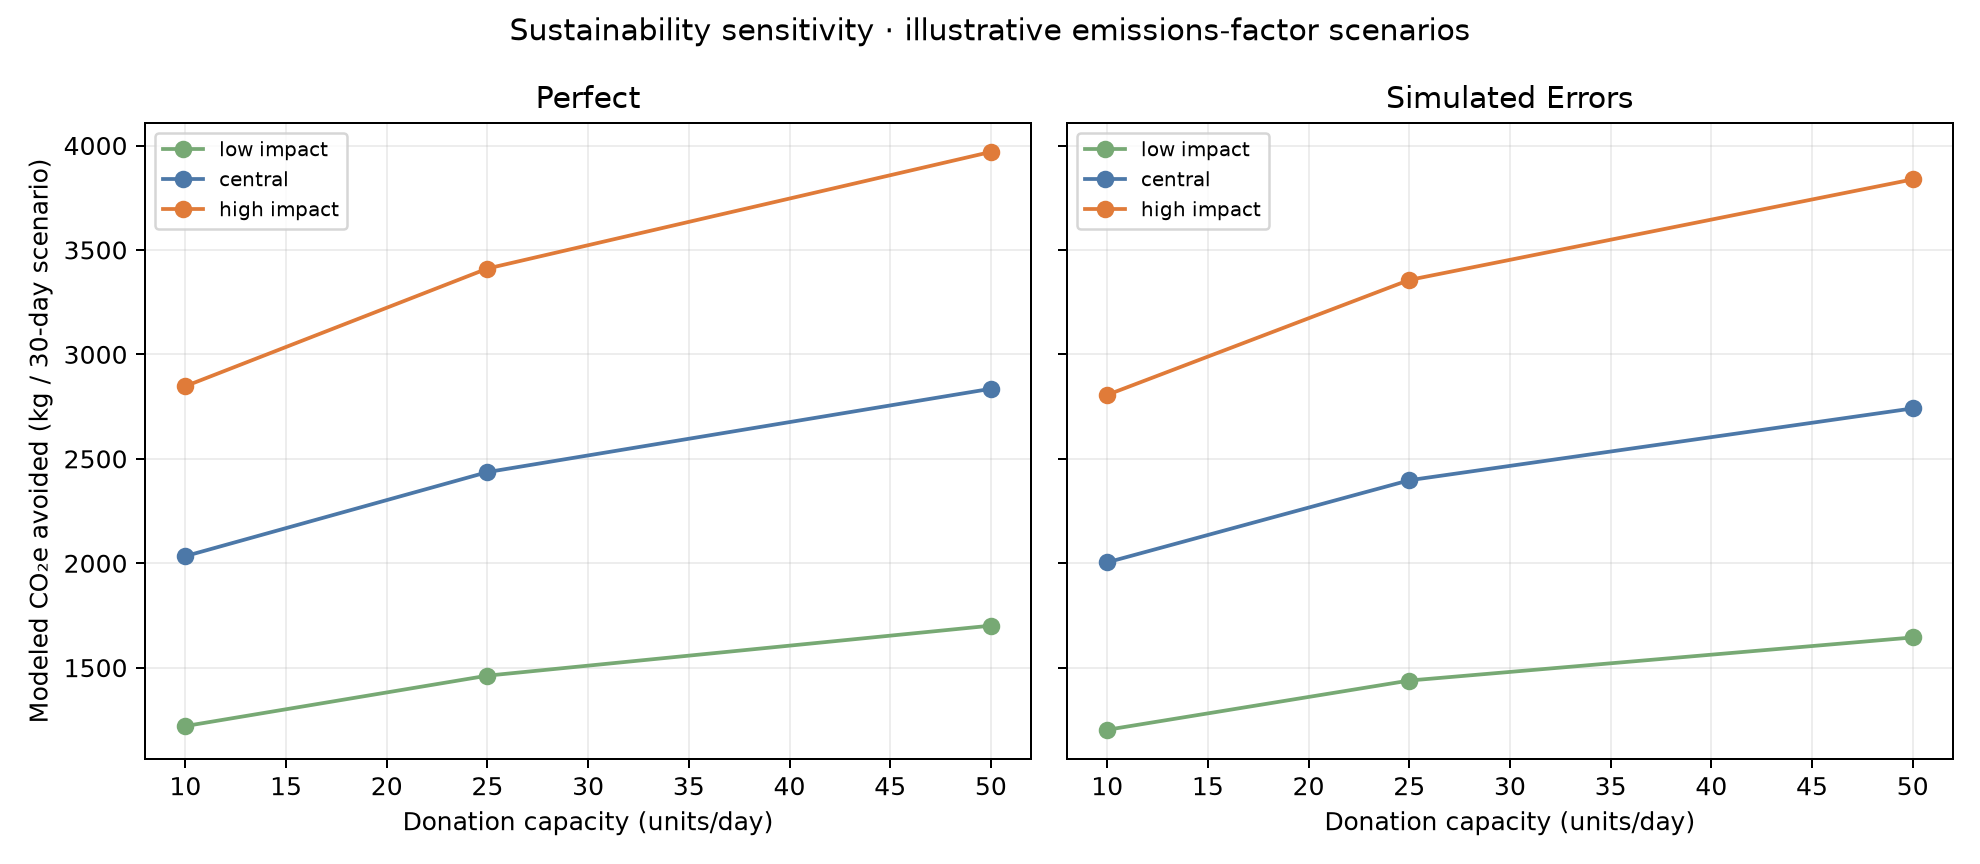
\includegraphics[width=0.96\textwidth]{sustainability_impact_sensitivity.png}
\caption{Modeled CO$_2$e sensitivity using the three illustrative factors. Values inherit inventory-model assumptions and are not measured climate benefits.}
\label{fig:sustainability}
\end{figure*}

\section{Sustainability and SDG Impact}
The proposed pathway is conditional: correct identification may route eligible near-expiry products to donation or discount before expiry. The L1, capacity-25 model yields 19.544 fewer mean saved units under simulated errors than under perfect recognition, while mean expired stock increases by 8.966. This comparison is specific to configured class proportions, confusion probabilities, queue rules, and recovery.

The conceptual mapping to UN SDG 12, Target 12.3, is not an indicator measurement \cite{sdg12}. The SDG 13 mapping is similarly contextual \cite{sdg13}. The calculation is
\begin{equation}
M_{\text{food}}=U_{\text{saved}}m_u,\qquad
E_{\text{potential}}=M_{\text{food}}f,
\end{equation}
where $U_{\text{saved}}$ is the model's defined saved-unit count, $m_u=0.8$ kg/unit is assumed, and $f$ is a configured kg CO$_2$e/kg factor. Upstream production, refrigeration, transport, packaging, donation logistics, and displacement effects are omitted; therefore the estimate is not net mitigation or a life-cycle assessment. No Nigam formula or factor is used.

\section{Discussion}
\subsection{Assessment evidence and interpretation}
\textit{Methodological novelty:} The contribution is integration of Blender RGB context, computational colour comparison, a synthetic print transfer, an assumed observer, and an alternative donation-capacity model. It is not a priority claim. The literature matrix marks unavailable full-text comparisons NV.

\textit{Retail applicability:} The supplied Nigam copy motivates the Near-Expiry failure mode. This project models red donation triggers and capacity but does not reuse Nigam equations or reproduce its results. A missed red action can leave an item outside the donation queue in the model; actual eligibility, staff practices, partner capacity, and stock disposition were not observed.

\textit{Rigour:} Configuration, seed, source CIE tables, software versions, 12 colour calculations, 10,000 synthetic trials per condition, 500 inventory replicates per scenario, results, and test logs are retained. Intervals describe this model and finite configured design; there is no participant sample, physical repeatability estimate, or human-inference test.

\textit{Sustainability:} Capacity and assumed mass/emissions calculations are explicit and auditable. Factors are illustrative; there is no sourced product footprint, LCA, SDG indicator evaluation, or realized impact.

\textit{Blender feasibility:} Two reproducible scenes are included. The controlled Cycles/Standard scene supplies 12 RGB render conditions; the six-camera presentation scene uses Cycles, denoising, and AgX. Python, not Blender pixels, supplies the spectral colorimetry. The GLB is visual only.

\subsection{Limitations}
\textit{Construct validity:} \dE{} compares a selected digital metamer with a synthetic absorbance transfer. The inverse is non-unique, and smoothness/substrate/density settings affect the result. A colour metric cannot represent text legibility, visual acuity, colour-vision variation, viewing distance, glare, or attention.

\textit{Illuminants:} D65 uses a recognized table. LED spectra are three-Gaussian approximations fitted to target Planckian chromaticity; they are not measured lamps. Blender uses RGB visualization, not spectral rendering.

\textit{Behaviour:} The logistic curve is selected, not fitted. The apparent relation between \dE{} and classification error is partly true by construction. Simulated misses and the logit do not predict employee or customer behaviour.

\textit{Inventory and impact:} Poisson arrivals, red fraction, horizon, capacities, recovery probability, and product mass are assumptions. The model lacks product-specific life, safety rules, sales, and logistics. Emissions factors are unsourced illustrative values.

\textit{Software:} Logs evidence local execution, not security certification or production readiness. Application allow-lists and bounded requests were tested; Docker and cloud deployment remain unverified. No claim of authentication, high availability, backup recovery, or cloud-scale performance is made.

Future validation requires measured reflectance for real label materials, spectral data for store lamps, and an approved human-perception study before behavioral calibration. Retail capacity and arrival parameters should come from documented operational data. A traceable product-category emission factor and lifecycle boundary are needed before making environmental impact claims.


\section{Conclusion}
This paper reports a software-only system that calculates CIEDE2000 differences between configured digital colours and a synthetic virtual-print response under tabulated D65 and two parameterized LED spectra, then propagates those outputs through assumed observer and inventory models. Red \texttt{\#D62828} produces calculated \dE{} values 1.8765, 2.0521, and 2.0355 under D65, neutral LED, and warm LED. Simulated miss proportions are 5.46\%, 5.62\%, and 5.58\%. Under L1 and capacity 25/day, the model reports 1218.224 versus 1198.680 mean saved units for perfect recognition and simulated errors. These are reproducible outputs under stated assumptions, not physical or human findings. Measured spectra, empirical observer calibration, retail data, and sourced environmental factors are needed before real-world prediction or impact can be claimed.

\appendices
\section{Software-Engineering Diagrams}
The UML class and runtime object views are in Fig.~\ref{fig:uml}; the sequence and data-flow views are in Fig.~\ref{fig:sequence}. The deployment view is Fig.~\ref{fig:deployment}. The object diagram depicts a representative configured comparison. The component and data-flow diagrams reflect the client/API/scientific engine/SQLite/artifact boundaries. The deployment diagram is prepared topology only; Docker/cloud execution is unverified.

\begin{figure*}[!t]\centering
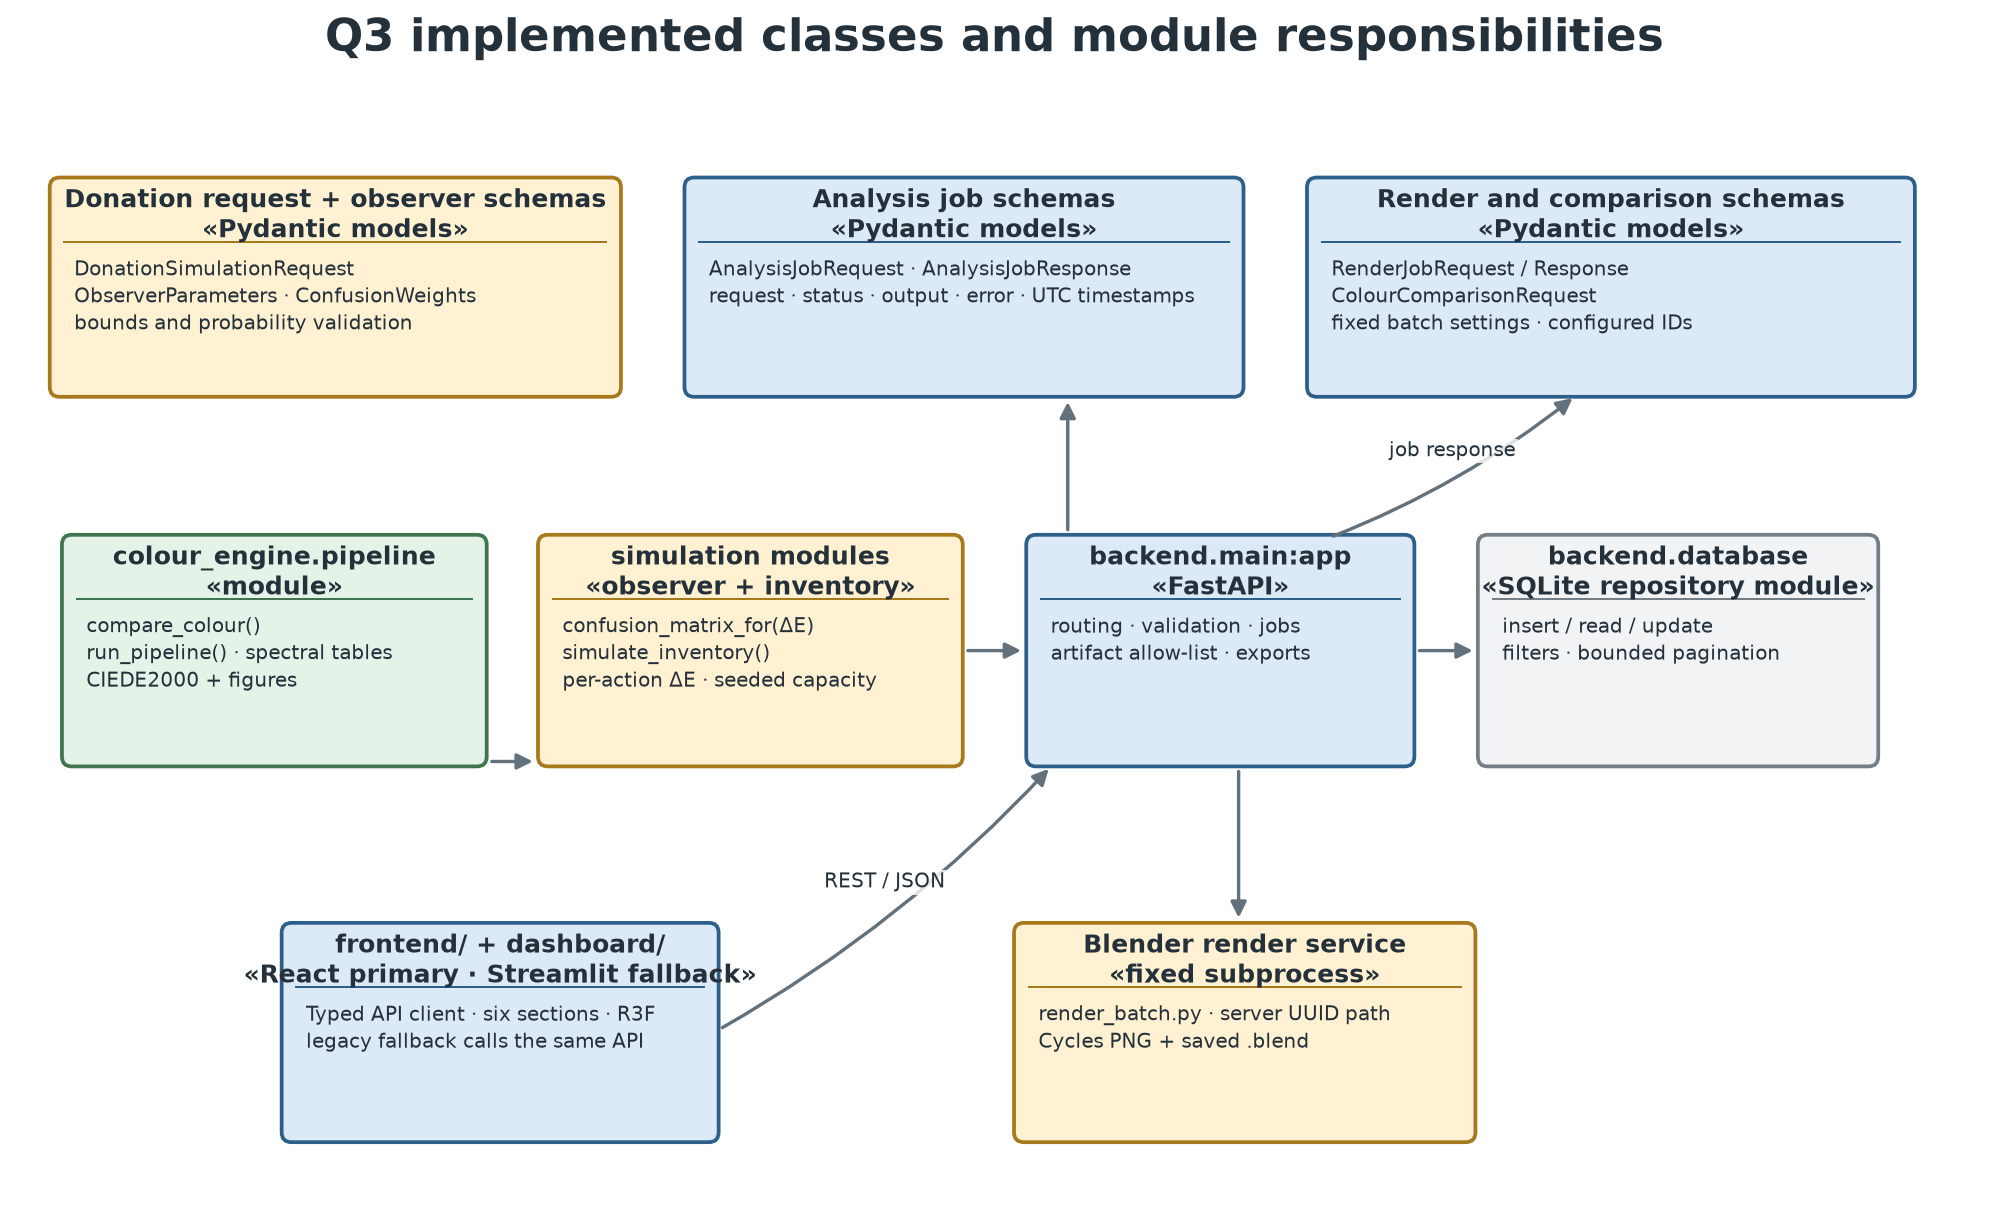
\includegraphics[width=0.96\textwidth,height=0.36\textheight,keepaspectratio]{class_diagram.png}\\[3pt]
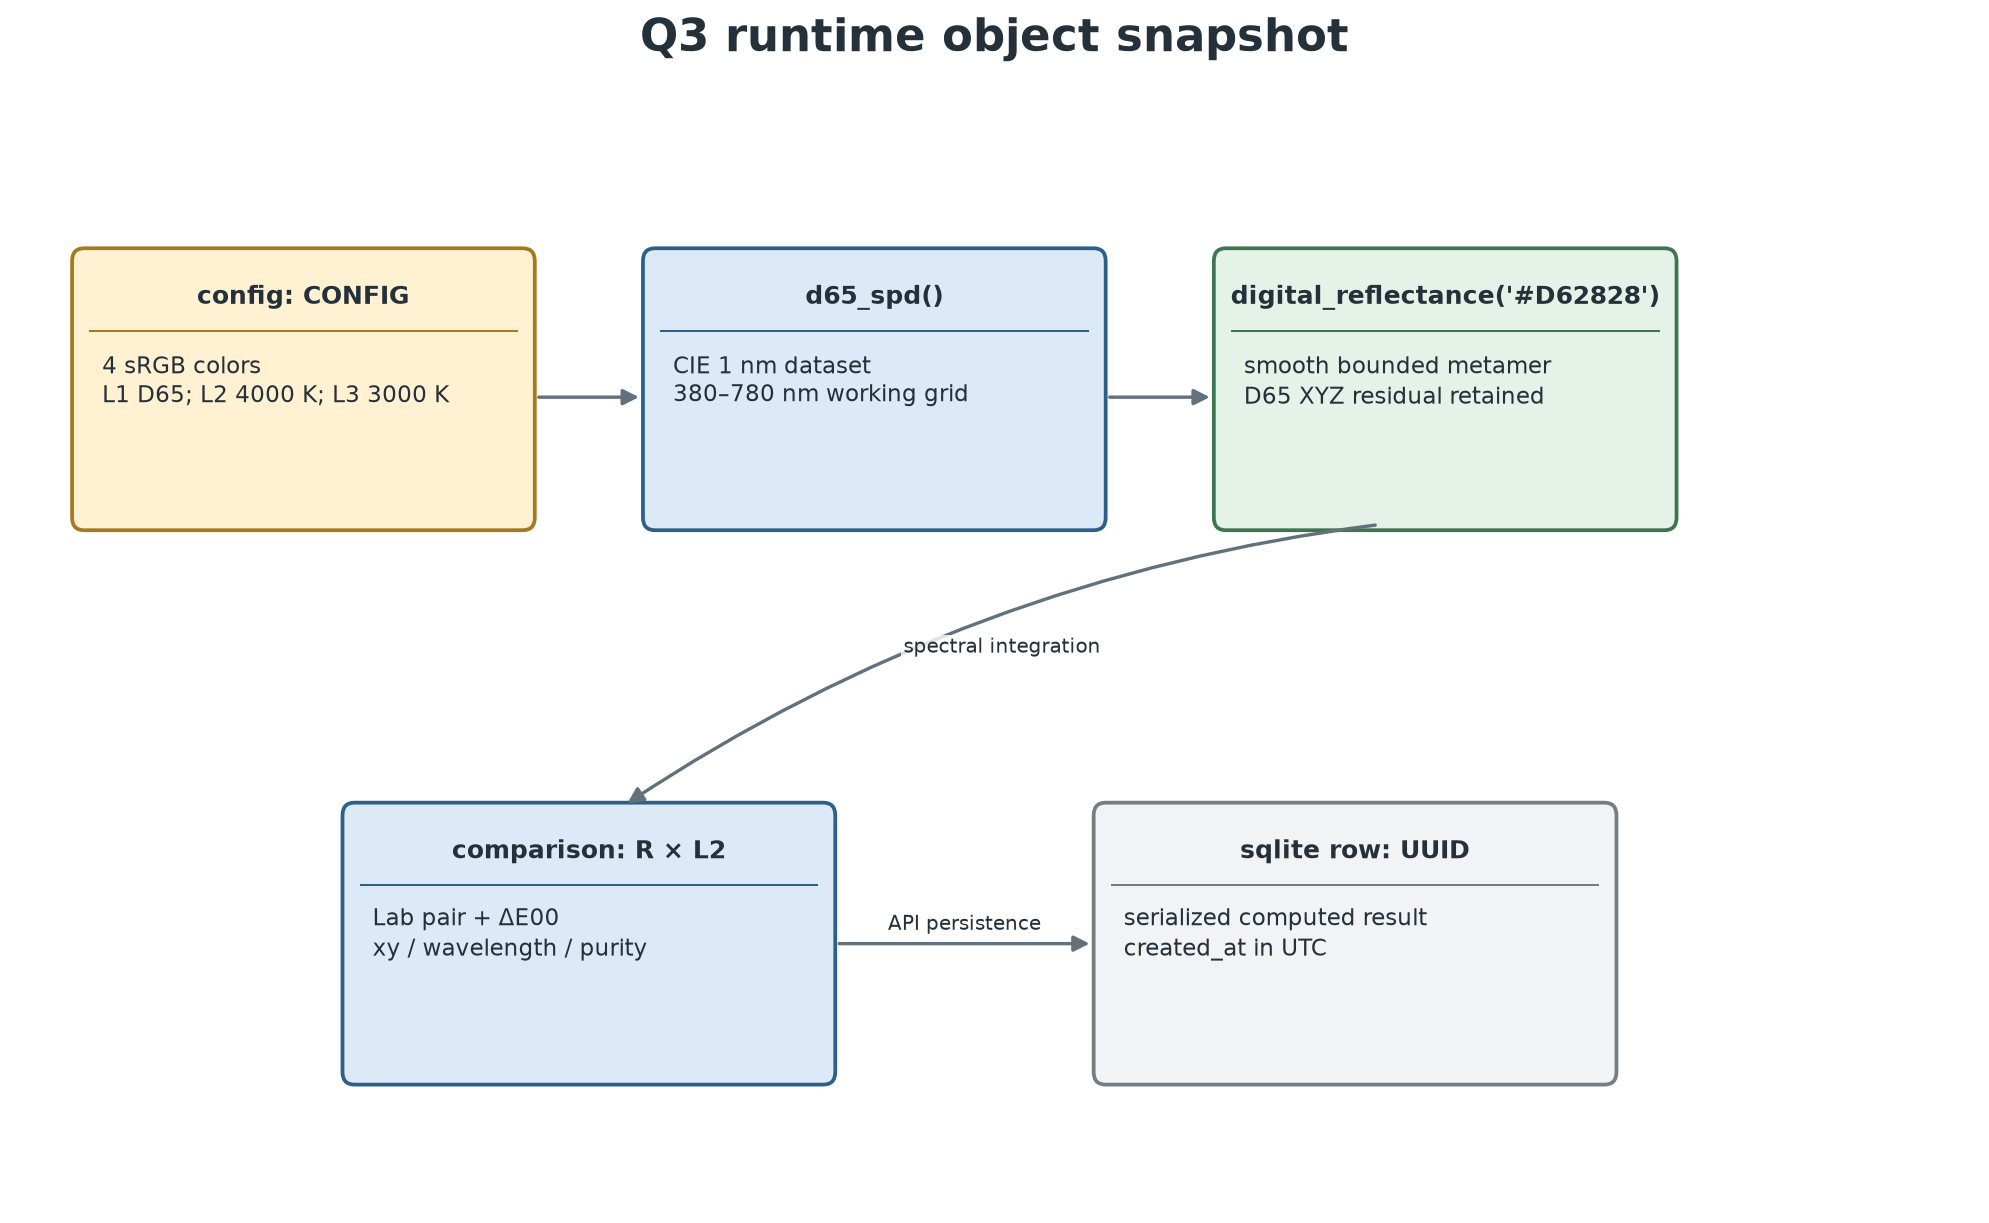
\includegraphics[width=0.96\textwidth,height=0.36\textheight,keepaspectratio]{object_diagram.png}
\caption{UML evidence: implemented class/API boundary structure (top) and a representative runtime object (bottom).}
\label{fig:uml}
\end{figure*}
\begin{figure*}[!t]\centering
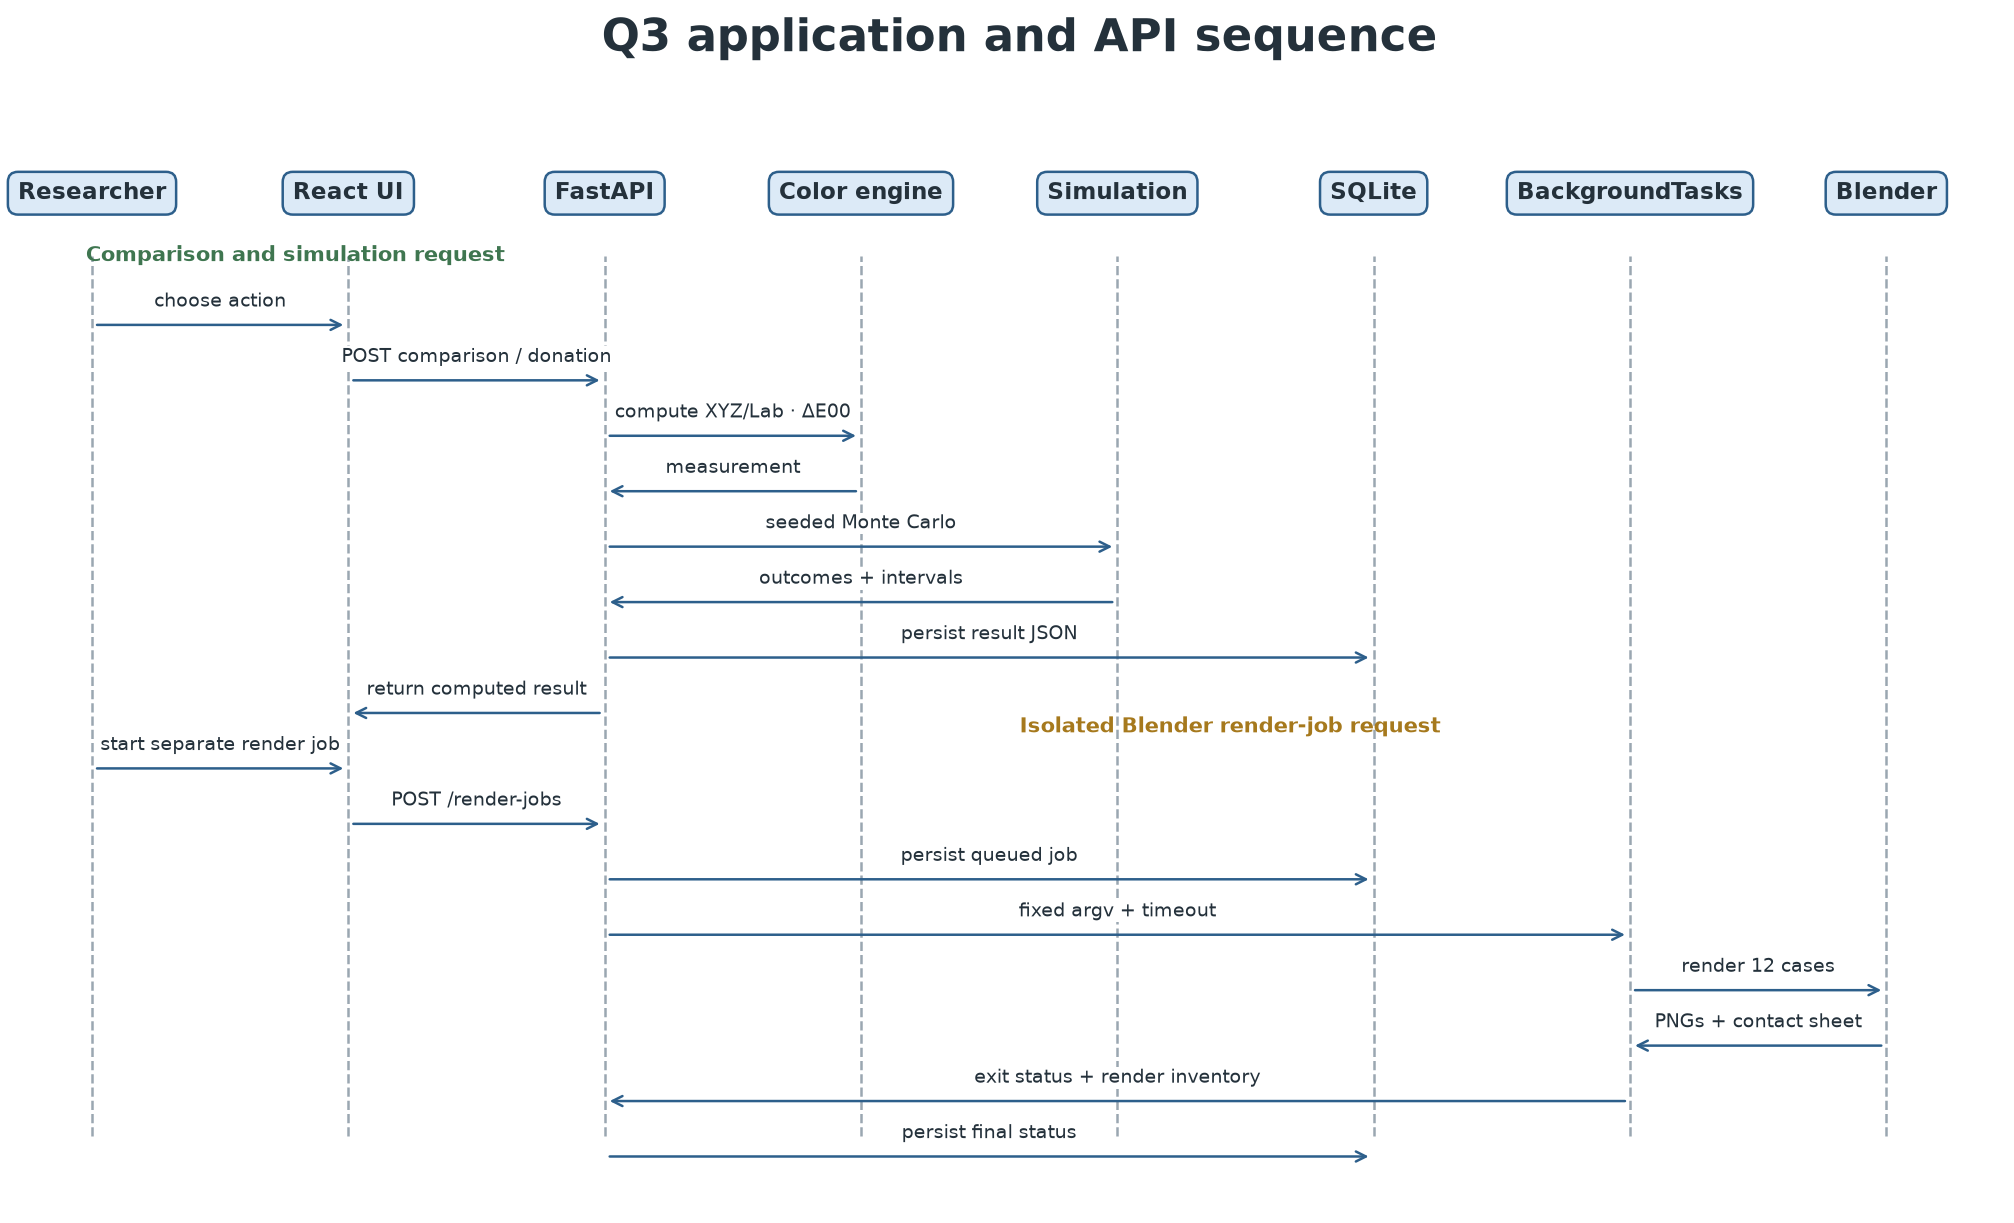
\includegraphics[width=0.96\textwidth,height=0.36\textheight,keepaspectratio]{sequence_diagram.png}\\[3pt]
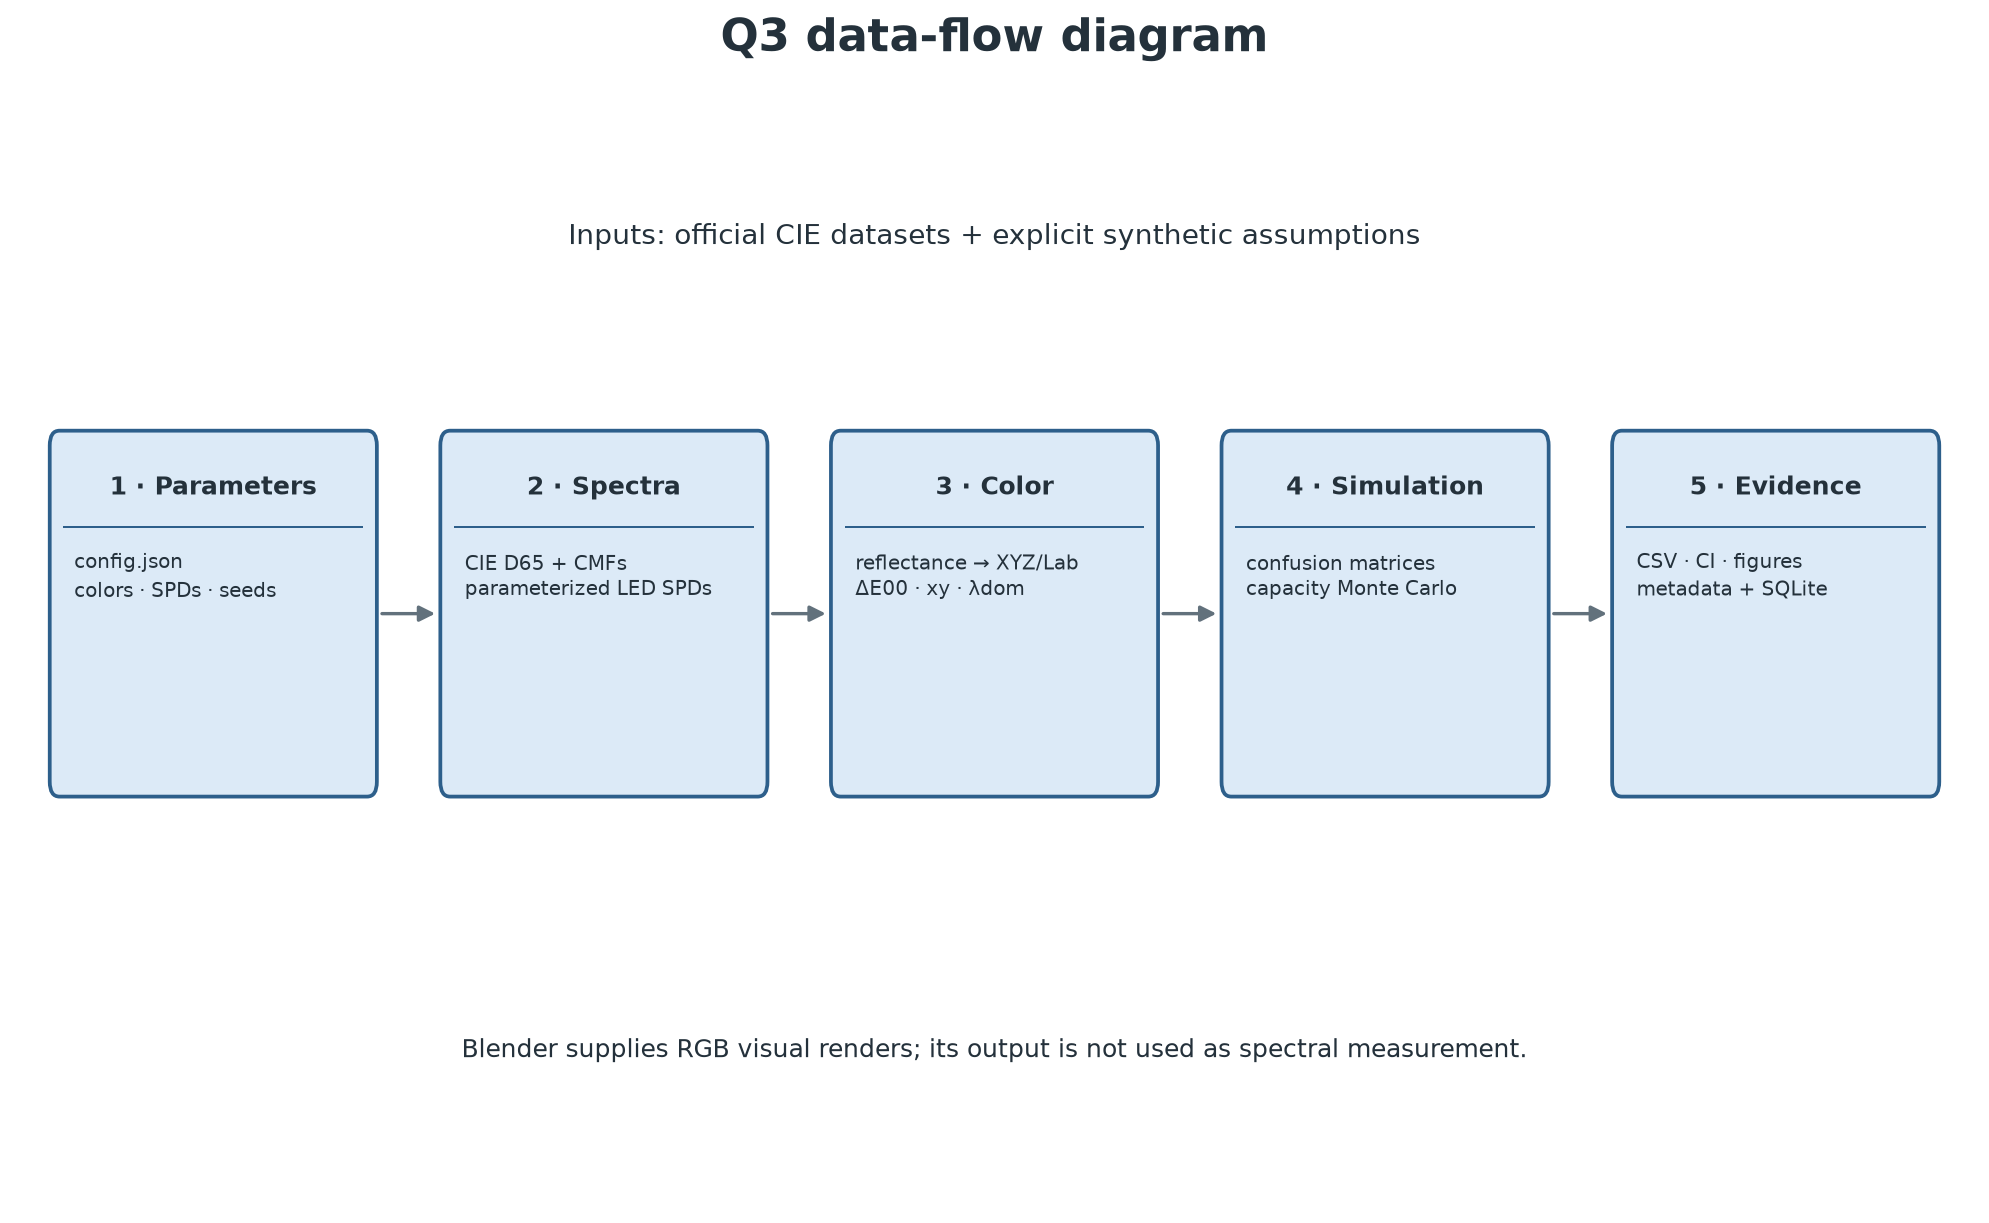
\includegraphics[width=0.96\textwidth,height=0.36\textheight,keepaspectratio]{data_flow_diagram.png}
\caption{Sequence diagram (top) and data-flow diagram (bottom) for API-backed computation and artifact handling.}
\label{fig:sequence}
\end{figure*}
\begin{figure*}[!t]\centering
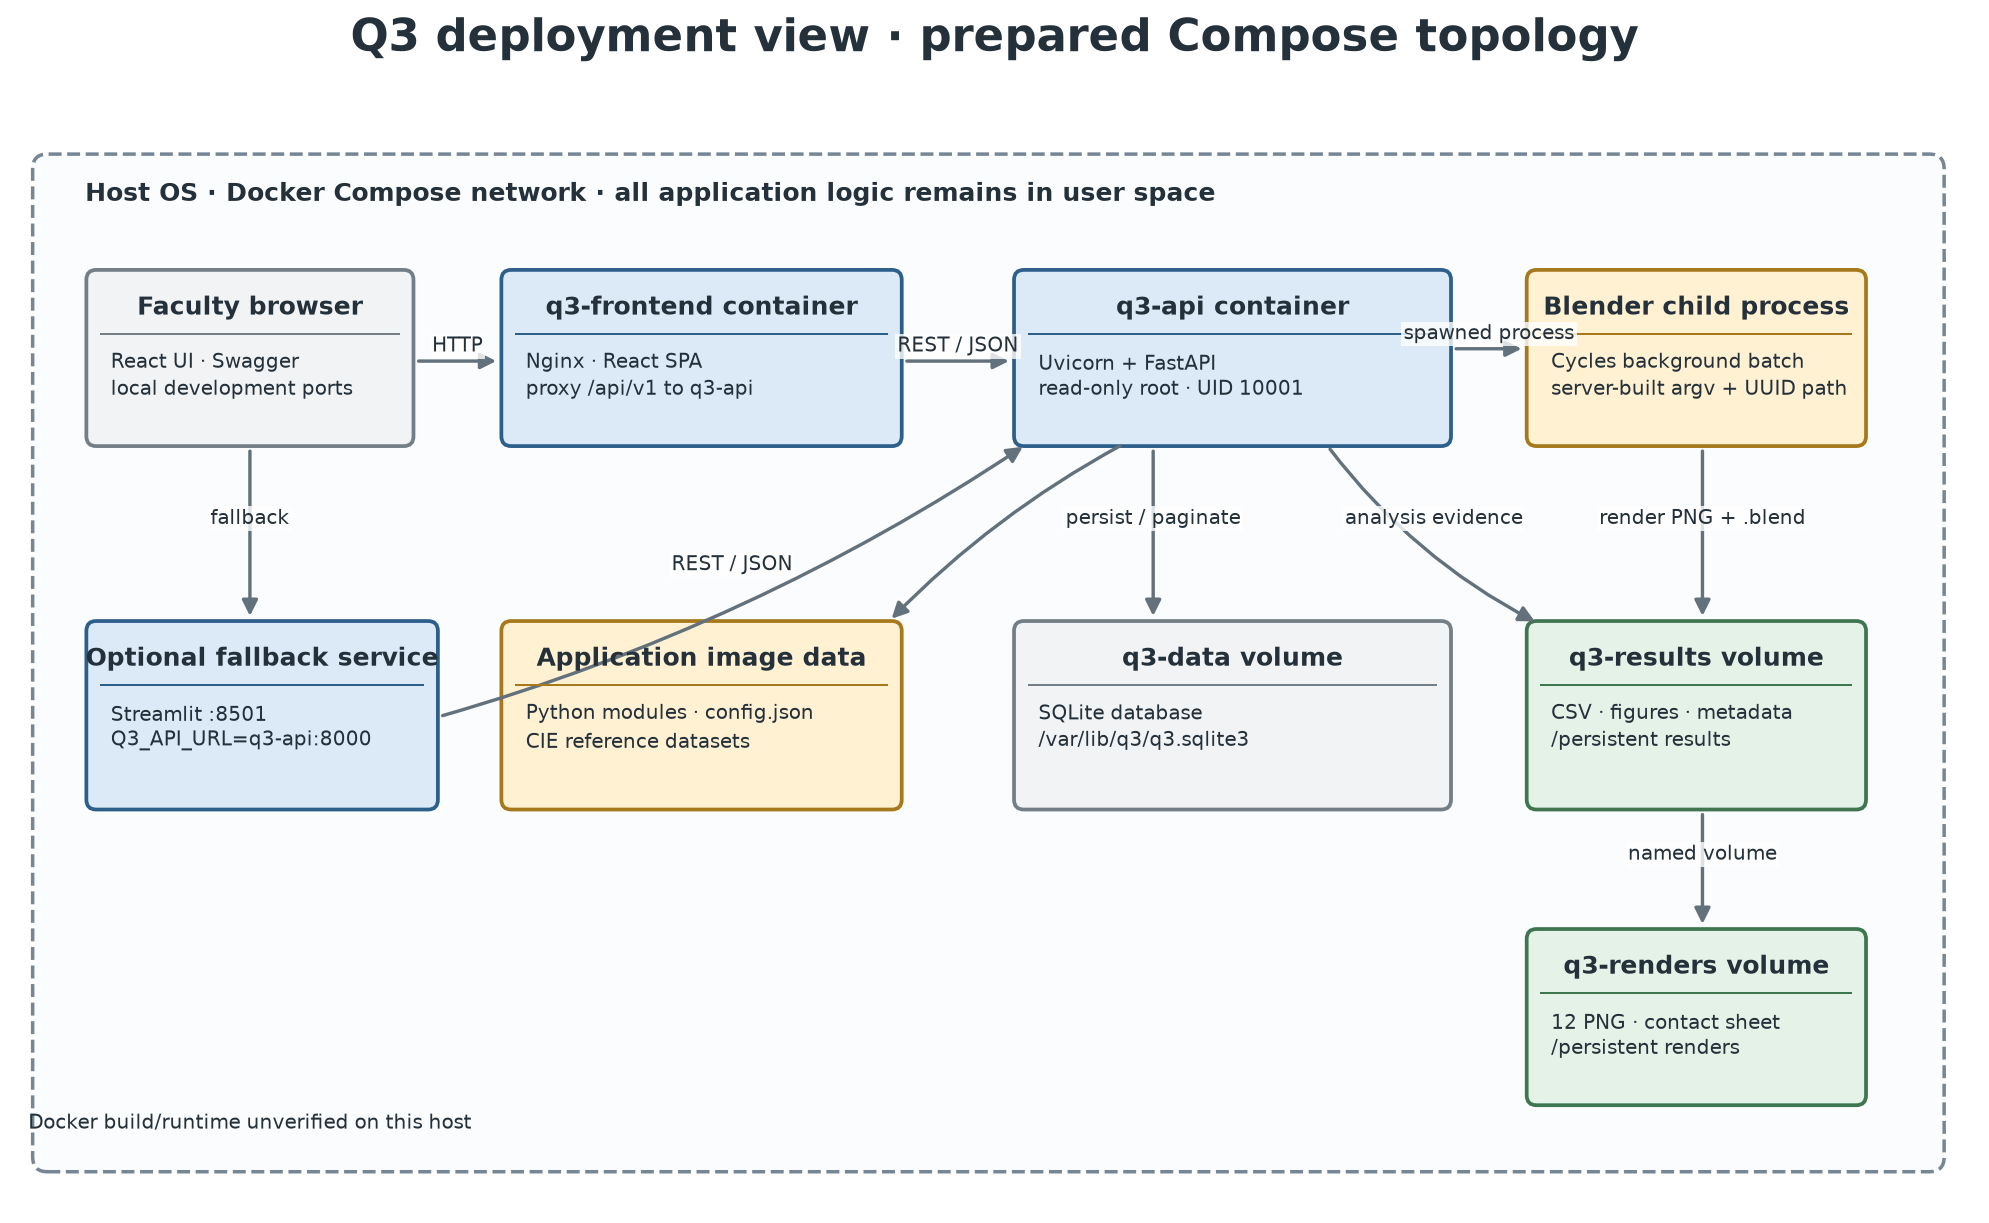
\includegraphics[width=0.96\textwidth]{deployment_diagram.png}
\caption{Prepared deployment topology; it is not evidence of successful container or cloud deployment.}
\label{fig:deployment}
\end{figure*}

\section{API Routing, Pagination, and Request Controls}
The REST base is \texttt{/api/v1}. Health is \texttt{GET /health}. Render and analysis jobs use POST submission, GET collection history, and GET item status routes. Colour comparisons and donation simulations support create, collection, and item routes. Collections accept bounded \texttt{limit} (default 50, 1--200), nonnegative \texttt{offset}, and applicable filters: \texttt{status}, \texttt{illumination\_id}, and \texttt{recognition}. Responses include \texttt{total}, \texttt{limit}, \texttt{offset}, and \texttt{items}; Swagger/OpenAPI is generated by FastAPI.

Sandbox tests cover safe file routing, bounded computation, no caller-selected output path, and fixed artifact allow-lists. They do not establish isolation from OS vulnerabilities or malicious native code. The container configuration applies an unprivileged user and filesystem/capability restrictions, but it was not executed in the recorded run.

\section{Research Evidence}
The accompanying \texttt{data/} directory contains final colour measurements and summaries, chromaticity, trigger trials and rates, the generated logistic diagnostic, donation Monte Carlo results, statistical summaries, sustainability scenarios, spectral tables, configuration, run metadata, and copied Phase 4 test logs. The \texttt{figures/} directory contains analytical charts, all 12 controlled measurement renders, six presentation renders, architecture/UML diagrams, and recorded dashboard screenshots. Original CSV names and relationships are preserved. Tables and the manuscript-specific inventory chart are generated from the copied CSVs by the scripts in \texttt{scripts/}.

\clearpage
\bibliographystyle{IEEEtran}
\bibliography{references}
\balance
\end{document}

